\chapter{李代数}

\section{李代数的定义}

\subsection{代数}

设 \(\mathbf{M}\) 是 \(\mathbf{K}\) 上的含单位元模，并带有一个双线性映射 \((x,y)\mapsto xy\)，它从 \(\mathbf{M}\times \mathbf{M}\) 到 \(\mathbf{M}\)。除乘法的结合律外，代数的所有公理都满足。滥用术语，称 \(\mathbf{M}\) 为 \(\mathbf{K}\) 上不必结合的代数；有时在不会引起混淆时，也简称为 \(\mathbf{K}\) 上的代数。本号中采用后一种记法。

若在 K-模 M 上赋予乘法 \((x,y)\mapsto yx\)，便得到一个代数，称为上述代数的逆代数。

M 的一个在乘法下稳定的子 K-模 N 以显然的方式成为 K 上的代数。称 N 为 M 的子代数。如果 \(x \in N\)、\(y \in M\) 蕴含 \(yx \in N\)（分别为 \(xy \in N\)），则称 N 为 M 的左（分别为右）理想。如果 N 既是左理想又是右理想，则称 N 为 M 的双边理想。在这种情形，利用 M 上的乘法，取商后可在商模 M/N 上定义双线性乘法，使 M/N 具有代数结构。称 M/N 为 M 关于 N 的商代数。

设 \(\mathbf{M}_1\) 和 \(\mathbf{M}_2\) 是 \(\mathbf{K}\) 上的两个代数，\(\phi\) 是从 \(\mathbf{M}_1\) 到 \(\mathbf{M}_2\) 的映射。称 \(\phi\) 为同态，当且仅当 \(\phi\) 是 K-线性的，并且 \(\phi(xy) = \phi(x)\phi(y)\) 对 \(x\in \mathbf{M}_1\)、\(y\in \mathbf{M}_1\) 成立。\(\mathbf{N}\) 是 \(\phi\) 的核，且是 \(\mathbf{M}_1\) 的双边理想；\(\phi\) 的像是 \(\mathbf{M}_2\) 的子代数。取商后，\(\phi\) 定义了从代数 \(\mathbf{M}_1 / N\) 到代数 \(\phi (\mathbf{M}_1)\) 的同构。

设 \(\mathbf{M}\) 是 \(\mathbf{K}\) 上的代数。映射 \(\mathbf{D}\) 从 \(\mathbf{M}\) 到 \(\mathbf{M}\)，称为 \(\mathbf{M}\) 的导子，若它是 \(\mathbf{K}\)-线性的，并且 \(\mathrm{D}(xy) = (\mathrm{D}x)y + x(\mathrm{D}y)\) 对所有 \(x \in \mathbf{M}\) 和 \(y \in \mathbf{M}\) 成立。这个定义推广了 Algebra, Chapter IV, § 4, no. 3 中的定义 3。\(\mathbf{M}\) 的导子的核是 \(\mathbf{M}\) 的子代数。如果 \(\mathrm{D}_1\) 和 \(\mathrm{D}_2\) 是 \(\mathbf{M}\) 的导子，则 \(\mathrm{D}_1\mathrm{D}_2 - \mathrm{D}_2\mathrm{D}_1\) 也是 \(\mathbf{M}\) 的导子（参见 Algebra, Chapter IV, § 4, no. 3, Proposition 5；该命题的证明不使用代数的结合律）。

设 \(\mathbf{M}_1\) 和 \(\mathbf{M}_2\) 是 K 上的两个代数。在积 K-模 \(\mathbf{M} = \mathbf{M}_1 \times \mathbf{M}_2\) 上规定乘法如下：

\[
(x _ {1}, x _ {2}) (y _ {1}, y _ {2}) = (x _ {1} y _ {1}, x _ {2} y _ {2}),
\]

对所有满足 \(x_1, y_1\) 属于 \(\mathbf{M}_1, x_2, y_2\) 属于 \(\mathbf{M}_2\) 的情形，如此定义的代数称为 \(\mathbf{M}_1\) 和 \(\mathbf{M}_2\) 的积代数。映射 \(x_1 \mapsto (x_1, 0)\)（分别为 \(x_2 \mapsto (0, x_2)\)）将 \(\mathbf{M}_1\)（分别为 \(\mathbf{M}_2\)）同构到 M 的一个双边理想上。在这些同构下，把 \(\mathbf{M}_1\) 和 \(\mathbf{M}_2\) 视为 M 的双边理想。于是 K-模 M 是 \(\mathbf{M}_1\) 与 \(\mathbf{M}_2\) 的直和。反之，设 M 是 K 上的代数，\(\mathbf{M}_1, \mathbf{M}_2\) 是 M 的两个双边理想，且 M 是 \(\mathbf{M}_1\) 与 \(\mathbf{M}_2\) 的直和。则 \(\mathbf{M}_1\mathbf{M}_2 \subset \mathbf{M}_1 \cap \mathbf{M}_2 = \{0\}\)；于是若 \(x_1, y_1\) 属于 \(\mathbf{M}_1\)，\(x_2, y_2\) 属于 \(\mathbf{M}_2\)，则 \((x_1 + x_2)(y_1 + y_2) = x_1y_1 + x_2y_2\)，从而可将 M 视为积代数 \(\mathbf{M}_1 \times \mathbf{M}_2\)。\(\mathbf{M}_1\) 的每个左（分别为右、双边）理想都是 M 的左（分别为右、双边）理想。任意有限族代数的情形中相应结果如何表述，留给读者完成。

设 \(\mathbf{M}\) 是 \(\mathbf{K}\) 上的代数，并设 \(\mathbf{K}\)-模 \(\mathbf{M}\) 有一个基 \((a_{\lambda})_{\lambda \in \mathbf{L}}\)。存在唯一的系统 \((\gamma_{\lambda \mu \nu})_{(\lambda, \mu, \nu) \in \mathbf{L} \times \mathbf{L} \times \mathbf{L}}\)，其元素属于 \(\mathbf{K}\)，并满足 \(a_{\lambda}a_{\mu} = \sum_{\nu} \gamma_{\lambda \mu \nu}a_{\nu}\) 对 \(\lambda, \mu\) 属于 \(\mathbf{L}\) 成立。称 \(\gamma_{\lambda \mu \nu}\) 为 \(\mathbf{M}\) 关于基 \((a_{\lambda})\) 的结构常数。

设 \(\mathbf{M}\) 是 \(\mathbf{K}\) 上的代数，\(\mathbf{K}_0\) 是含单位元的交换环，\(\rho\) 是将单位元映到单位元的从 \(\mathbf{K}_0\) 到 \(\mathbf{K}\) 的同态。则可将 \(\mathbf{M}\) 视为 \(\mathbf{K}_0\) 上的代数，规定 \(\alpha.x = \rho(\alpha).x\)（其中 \(\alpha \in \mathbf{K}_0, x \in \mathbf{M}\)）。特别地，当 \(\mathbf{K}_0\) 是含单位元的 \(\mathbf{K}\) 的子环，并取 \(\rho\) 为 \(\mathbf{K}_0\) 到 \(\mathbf{K}\) 的包含映射时，正是这种情形。

设 M 是 K 上的代数，\(K_{1}\) 是含单位元的交换环，\(\sigma\) 是将单位元映到单位元的从 K 到 \(K_{1}\) 的同态。令 \(M_{(K_{1},\sigma)} = M_{(K_{1})}\) 表示 \(K_{1}\)-模，即由 M 将标量环扩张到 \(\mathbf{K}_1\) 后得到的模（参见 Algebra, Chapter II, § 5）。M 上的乘法自然定义了一个 \(\mathbf{K}_1\)-双线性映射，从 \(\mathrm{M}_{(\mathbf{K}_1)} \times \mathrm{M}_{(\mathbf{K}_1)}\) 到 \(\mathrm{M}_{(\mathbf{K}_1)}\)（参见 Algebra, Chapter IX, § 1, no. 4），使 \(\mathrm{M}_{(\mathbf{K}_1)}\) 具有 \(\mathbf{K}_1\) 上的代数结构（称为由 M 将标量环扩张到 \(\mathbf{K}_1\) 后得到的代数）。特别地，当 K 是含单位元的 \(\mathbf{K}_1\) 的子环，且 \(\sigma\) 是 K 到 \(\mathbf{K}_1\) 的包含映射时，也是这种情形。

\subsection{李代数}

定义 1. 如果 K 上的代数 g 的乘法（记作 \((x,y)\mapsto [x,y])\) 满足下列恒等式，则称 g 为 K 上的李代数：

\[
[ x, x ] = 0\tag{1}
\]

\[
[ x, [ y, z ] ] + [ y, [ z, x ] ] + [ z, [ x, y ] ] = 0\tag{2}
\]

对 g 中所有 x, y, z 均成立。

乘积 \([x, y]\) 称为 \(x\) 与 \(y\) 的括号。恒等式 (2) 称为 Jacobi 恒等式。

括号 \([x, y]\) 是关于 \(x\) 和 \(y\) 的交错双线性函数。我们有恒等式：

\[
[ x, y ] = - [ y, x ]\tag{3}
\]

因此 Jacobi 恒等式可写为：

\[
[ x, [ y, z ] ] = [ [ x, y ], z ] + [ y, [ x, z ] ].\tag{4}
\]

李代数的每个子代数和商代数都是李代数。李代数的每个积代数也是李代数。若 g 是李代数，则逆代数 \(g^{0}\) 也是李代数，并且由恒等式 (3)，映射 \(x \mapsto -x\) 是从 g 到 \(g^{0}\) 的同构。

例 1. 设 L 是 K 上的结合代数。括号 \([x, y] = xy - yx\) 是关于 \(x\) 和 \(y\) 的双线性函数。容易验证，在 K-模 L 上定义的复合律 \((x, y) \mapsto [x, y]\) 使 L 成为 K 上的李代数。

例 2. 在例 1 中，取 L 为 K-模 E 的自同态组成的结合代数。得到 E 的自同态李代数，记作 \(\mathfrak{gl}(\mathbf{E})\)。（若 \(\mathbf{E} = \mathbf{K}^n\)，则李代数 \(\mathfrak{gl}(\mathbf{E})\) 记作 \(\mathfrak{gl}(n, \mathbf{K})\)。）

\(\mathfrak{gl}(\mathbf{E})\) 的每个李子代数都是 K 上的李代数。特别地：

\begin{enumerate}
\def\labelenumi{(\arabic{enumi})}
\item
  若 E 赋有（不必结合的）代数结构，则 E 的导子构成 K 上的李代数。
\item
  若 E 有限维，则 E 的零迹自同态构成 K 上的李代数，记作 \(\mathfrak{sl}(\mathbf{E})\)（或者记作 \(\mathfrak{sl}(n,\mathbf{K})\)，若 \(E = K^{n}\)）。
\item
  方阵集合 \(\mathbf{M}_n(\mathbf{K})\)（其阶为 \(n\)）可视为 K 上的李代数，并且与 \(\mathfrak{gl}(n, \mathbf{K})\) 有自然同构。令 \((E_{ij})\) 为 \(\mathbf{M}_n(\mathbf{K})\) 的典范基（Algebra, Chapter II, § 10, no. 3）。容易得到：
\end{enumerate}

\[
\left\{ \begin{array}{l l} [ E _ {i j}, E _ {k l} ] = 0 & \text {if} j \neq k \quad \text {and} \quad i \neq l \\ {} [ E _ {i j}, E _ {j l} ] = E _ {i l} & \text {if} i \neq l \\ {} [ E _ {i j}, E _ {k i} ] = - E _ {k j} & \text {if} j \neq k \\ {} [ E _ {i j}, E _ {j i} ] = E _ {i i} - E _ {j j} \end{array} \right.\tag{5}
\]

由三角矩阵（分别为零迹三角矩阵、零对角线三角矩阵）组成的 \(\mathbf{M}_{n}(\mathbf{K})\) 的李子代数记作 \(t(n,\mathbf{K})\)（分别记作 \(\mathfrak{st}(n,\mathbf{K})\)、\(\mathfrak{n}(n,\mathbf{K})\)）（Algebra, Chapter II, § 10, no. 7）。

*例 3. 设 V 是无穷可微实流形。具有无穷可微实系数的微分算子构成 R 上的结合代数，因此由例 1 得到 R 上的李代数 \(\Delta\)。V 上两个无穷可微向量场的括号仍是无穷可微向量场，所以 V 上的无穷可微向量场构成李子代数 \(\mathfrak{f}\)，它是 \(\Delta\) 的子代数。若 V 是实李群，则左不变向量场构成李子代数 \(\mathfrak{g}\)，它是 \(\mathfrak{f}\) 的子代数，称为 V 的李代数。向量空间 \(\mathfrak{g}\) 与 V 在 \(e\) 处的切空间相同（V 的单位元）。设 V' 是另一个实李群，\(e'\) 是其单位元，\(\mathfrak{g}'\) 是其李代数。V 到 V' 的每个解析同态都定义了从 V 在 \(e\) 处的切空间到 V' 在 \(e'\) 处的切空间的线性映射；该映射是从李代数 \(\mathfrak{g}\) 到李代数 \(\mathfrak{g}'\) 的同态。若 V 是有限维实向量空间 E 的线性群，则存在从 gl(E) 到 V 的李代数 \(\mathfrak{g}\) 的典范同构，在此同构下 \(\mathfrak{g}\) 与 gl(E) \(_*\) 相同。*

定义 2. 设 g 是李代数，x 是 g 的元素。从 g 到 g 的线性映射 \(y \mapsto [x, y]\) 称为 x 的伴随线性映射，记作 \(ad_{g}x\) 或 ad x。

命题 1. 设 \(\mathfrak{g}\) 是李代数。对所有 \(x \in \mathfrak{g}\)，ad \(x\) 都是导子。映射 \(x \mapsto \operatorname{ad} x\) 是从李代数 \(\mathfrak{g}\) 到导子李代数 \(\mathfrak{d}\)（由 \(\mathfrak{g}\) 的导子组成）的同态。若 \(\mathrm{D} \in \mathfrak{d}\) 且 \(x \in \mathfrak{g}\)，则 {[}D, ad \(x\) {]} = \(\operatorname{ad}(\mathrm{D}x)\)。

恒等式 (4) 可写为：

\[
(\operatorname{ad} x). [ y, z ] = [ (\operatorname{ad} x). y, z ] + [ y, (\operatorname{ad} x). z ]
\]

或写为：

\[
(\operatorname{ad} [ x, y ]). z = (\operatorname{ad} x). ((\operatorname{ad} y). z) - (\operatorname{ad} y). ((\operatorname{ad} x). z)
\]

由此得到前两个断言。另一方面，若 \(\mathbf{D} \in \mathfrak{d}\)、\(x \in \mathfrak{g}\)、\(y \in \mathfrak{g}\)，则 \([\mathbf{D}, \operatorname{ad} x] \cdot y = \mathrm{D}([x, y]) - [x, \mathrm{D}y] = [\mathrm{D}x, y] = (\operatorname{ad} \mathrm{D}x) \cdot y\)，从而得到最后一个断言。

映射 ad \(x\) 也称为由 \(x\) 定义的内导子。

\subsection{交换李代数}

定义 3. 李代数的两个元素 \(x, y\) 若满足 \([x, y] = 0\)，则称它们可交换。\(g\) 若其任意两个元素都可交换，则称为交换的。

例 1. 设 L 是结合代数，g 是由它定义的李代数（第 2 号，例 1）。g 中两个元素 x, y 可交换，当且仅当它们在 L 中满足 xy = yx。

*例 2. 若实李群 G 是交换的，则其李代数也是交换的。*

每个 K-模显然都能唯一地赋予 K 上的交换李代数结构。

若 g 是李代数，则 g 的每个单生成子模都是 g 的交换李子代数。

\subsection{理想}

由恒等式 (3) 可知，在李代数 \(\mathfrak{g}\) 中左理想与右理想没有区别，每个理想都是双边的。因此我们简称为理想。

*例. 设 G 是李群，g 是其李代数，H 是 G 的李子群。H 上每个左不变向量场都自然地定义 G 上的一个左不变向量场，从而 H 的李代数 h 自然嵌入 g；在此嵌入下，h 被视为 g 的李子代数。若 H 是 G 的正规子群，则 h 在 g 中的典范像是 g 的理想。*

g 的理想是 g 的一个在 g 的内导子下稳定的子模。

定义 4. g 的一个在 g 的每个导子下都稳定的子模称为 g 的特征理想。

命题 2. 设 g 是李代数，a 是 g 的理想（分别为特征理想），b 是 a 的特征理想。则 b 是 g 的理想（分别为特征理想）。

g 的每个内导子（分别为每个导子）都保持 a 稳定，并在 a 上诱导一个导子，因而保持 b 稳定。

设 \(\mathfrak{g}\) 是李代数。若 \(\mathfrak{a}\) 和 \(\mathfrak{b}\) 是 \(\mathfrak{g}\) 的理想，则 \(\mathfrak{a} + \mathfrak{b}\) 和 \(\mathfrak{a} \cap \mathfrak{b}\) 也是 \(\mathfrak{g}\) 的理想。

设 \(\mathfrak{a}\) 和 \(\mathfrak{b}\) 是 \(\mathfrak{g}\) 的两个子模。滥用记号，将 \(\mathfrak{g}\) 中由形如 \([x,y](x\in\mathfrak{a},y\in\mathfrak{b})\) 的元素生成的子模记作 \([\mathfrak{a},\mathfrak{b}]\)。由恒等式 (3)，有 \([\mathfrak{a},\mathfrak{b}] = [\mathfrak{b},\mathfrak{a}]\)。若 \(z\in\mathfrak{g}\)，则 \([z,\mathfrak{a}]\) 或 \([\mathfrak{a},z]\) 表示子模 \([\mathrm{K}z,\mathfrak{a}] = (\mathrm{ad}\,z)(\mathfrak{a})\)。

命题 3. 若 a 和 b 是 g 的理想（分别为特征理想），则 {[}a, b{]} 是 g 的理想（分别为特征理想）。

设 D 是 g 的内导子（分别为导子）。若 \(x \in a\) 且 \(y \in b\)，则

\[
\mathrm{D} ([ x, y ]) = [ \mathrm{D} x, y ] + [ x, \mathrm{D} y ] \in [ \mathfrak {a}, \mathfrak {b} ].
\]

故命题得证。

若 \(\mathfrak{a}\) 是 \(\mathfrak{g}\) 的子模，则由 \(x \in \mathfrak{g}\) 且满足 (ad \(x\) ). \(\mathfrak{a} \subset \mathfrak{a}\) 的元素组成的集合是一个子代数 \(\mathfrak{n}\)，属于 \(\mathfrak{g}\)，称为 \(\mathfrak{a}\) 在 \(\mathfrak{g}\) 中的正规化子。若进一步 \(\mathfrak{a}\) 是 \(\mathfrak{g}\) 的子代数，则 \(\mathfrak{a} \subset \mathfrak{n}\)，且 \(\mathfrak{a}\) 是 \(\mathfrak{n}\) 的理想。

\subsection{导出列与下中心列}

\([\mathfrak{g},\mathfrak{g}]\) 这一特征理想称为李代数 \(\mathfrak{g}\) 的导出理想，记作 \(\mathcal{D}\mathfrak{g}\)。

包含 \(\mathcal{D}\mathfrak{g}\) 的 g 的每个子模都是 g 的理想。

\(\mathfrak{g}\) 的导出列是递减序列 \(\mathcal{D}^0\mathfrak{g},\mathcal{D}^1\mathfrak{g},\ldots\)，其各项是 \(\mathfrak{g}\) 的特征理想，递归定义如下：(1) \(\mathcal{D}^0\mathfrak{g} = \mathfrak{g}\)；(2) \(\mathcal{D}^{p + 1}\mathfrak{g} = [\mathcal{D}^p\mathfrak{g},\mathcal{D}^p\mathfrak{g}]\)。

g 的下中心列是 g 的特征理想构成的递减序列 \(\mathcal{C}^1\mathfrak{g},\mathcal{C}^2\mathfrak{g},\ldots\)，递归定义如下：(1) \(\mathcal{C}^1\mathfrak{g} = \mathfrak{g}\)；(2) \(\mathcal{C}^{p + 1}\mathfrak{g} = [\mathfrak{g},\mathcal{C}^p\mathfrak{g}]\)。于是 \(\mathcal{C}^2\mathfrak{g} = \mathcal{D}\mathfrak{g}\)，并且 \(\mathcal{C}^{p + 1}\mathfrak{g}\supset \mathcal{D}^{p}\mathfrak{g}\) 对所有 \(p\) 都成立，这由对 \(p\) 的归纳立即可见。

命题 4. 设 \(\mathfrak{g}\) 和 \(\mathfrak{h}\) 是 \(\mathbf{K}\) 上的两个李代数，且 \(f\) 是从 \(\mathfrak{g}\) 到 \(\mathfrak{h}\) 上的满同态。则 \(f(\mathcal{D}^p\mathfrak{g}) = \mathcal{D}^{p}\mathfrak{h}, f(\mathcal{C}^p\mathfrak{g}) = \mathcal{C}^{p}\mathfrak{h}\)。

若 a 和 b 是 g 的子模，则立即得到

\[
f ([ \mathfrak {a}, \mathfrak {b} ]) = [ f (\mathfrak {a}), f (\mathfrak {b}) ].
\]

于是命题由对 p 的归纳立即得到。

推论. 设 g 是李代数，a 是 g 的理想。李代数 g/a 为交换的充要条件是 a ⊃ \(\mathcal{D}\mathfrak{g}\)。

说 \(\mathfrak{g} / \mathfrak{a}\) 是交换的，就是说 \(\mathcal{D}(\mathfrak{g} / \mathfrak{a}) = \{0\}\)。但根据命题 4，\(\mathcal{D}(\mathfrak{g} / \mathfrak{a})\) 正是 \(\mathcal{D}\mathfrak{g}\) 在 \(\mathfrak{g} / \mathfrak{a}\) 中的典范像。

\subsection{上中心列}

设 \(\mathfrak{g}\) 是李代数，\(\mathbf{P}\) 是 \(\mathfrak{g}\) 的子集。\(\mathbf{P}\) 在 \(\mathfrak{g}\) 中的中心化子是由 \(\mathfrak{g}\) 中与 \(\mathbf{P}\) 中元素可交换的元素组成的集合。此中心化子是所有 ad \(y\) 的核的交，其中 \(y\) 遍历 \(\mathbf{P}\)；因此它是 \(\mathfrak{g}\) 的子代数。

命题 5. 设 g 是李代数，a 是 g 的理想（分别为特征理想）。a 在 g 中的中心化子 \(\mathfrak{a}'\) 是 g 的理想（分别为特征理想）。

设 \(D\) 是 \(g\) 的内导子（分别为导子）。若 \(x \in a'\) 且 \(y \in a\)，则

\[
[ \mathrm{D} x, y ] = \mathrm{D} ([ x, y ]) - [ x, \mathrm{D} y ] = 0;
\]

因此 \(\mathrm{D}x\in \mathfrak{a}^{\prime}\)。故命题得证。

设 g 是李代数。g 在自身中的中心化子称为 g 的中心，即由 \(x \in g\) 满足 \([x, y] = 0\) 且对所有 \(y \in g\) 成立的元素构成的特征理想。g 的中心是同态 \(x \mapsto ad x\) 的核。

\(\mathfrak{g}\) 的上中心列是递增序列 \(\mathcal{C}_{0}\mathfrak{g},\mathcal{C}_{1}\mathfrak{g},\ldots\)，其各项是 \(\mathfrak{g}\) 的特征理想，递归定义如下：(1) \(\mathcal{C}_{0}\mathfrak{g} = \{0\}\)；(2) \(\mathcal{C}_{p + 1}\mathfrak{g}\) 是在从 \(\mathfrak{g}\) 到 \(\mathfrak{g} / \mathcal{C}_{p}\mathfrak{g}\) 的典范映射下，\(\mathfrak{g} / \mathcal{C}_{p}\mathfrak{g}\) 的中心的逆像。

理想 \(\mathcal{C}_{1}\mathfrak{g}\) 是 \(\mathfrak{g}\) 的中心。

\subsection{扩张}

定义 5. 设 \(\mathfrak{a}\) 和 \(\mathfrak{b}\) 是 \(\mathbf{K}\) 上的两个李代数。\(\mathfrak{b}\) 的 \(\mathfrak{a}\)-扩张是一个序列：

\[
a \xrightarrow {\lambda} g \xrightarrow {\mu} b
\]

其中 g 是 K 上的李代数，μ 是从 g 到 b 的满同态，λ 是将 a 同构到 μ 的核上的单同态。

扩张的核称为 \(\mathfrak{n}\)，即 \(\mu\) 的核。取商后，同态 \(\lambda\) 将 \(\mathfrak{a}\) 同构到 \(\mathfrak{n}\) 上，而同态 \(\mu\) 定义了从 \(\mathfrak{g} / \mathfrak{n}\) 到 \(\mathfrak{b}\) 的同构。

滥用术语，也称 g 为由 a 扩张 b。

两个扩张：

\[
a \xrightarrow {\lambda} g \xrightarrow {\mu} b, \quad a \xrightarrow {\lambda^ {\prime}} g ^ {\prime} \xrightarrow {\mu^ {\prime}} b
\]

若存在一个同态 \(f\)，它从 \(\mathfrak{g}\) 到 \(\mathfrak{g}'\)，使下图：

\pandocbounded{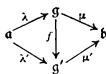
\includegraphics[keepaspectratio]{images/part001_2862d8fe.jpg}}

是交换的（即满足 \(f \circ \lambda = \lambda', \mu' \circ f = \mu\)），则称这两个扩张等价。我们说明这样的同态必为双射。首先 \(f\) 是单射。若 \(x \in \mathfrak{g}\) 满足 \(f(x) = 0\)，则 \(\mu(x) = \mu'(f(x)) = 0\)，从而 \(x = \lambda(y)\)，其中某个 \(y \in \mathfrak{a}\)；于是 \(\lambda'(y) = f(\lambda(y)) = f(x) = 0\)，故 \(y = 0\)，进而 \(x = 0\)。另一方面，\(f\) 是满射。因为 \(\mu' \circ f = \mu\) 是满射，所以 \(f(\mathfrak{g}) + \lambda'(\mathfrak{a}) = \mathfrak{g}'\)；另一方面 \(f(\mathfrak{g}) \supset f(\lambda(\mathfrak{a})) = \lambda'( \mathfrak{a})\)。

由此可知，刚才定义的两个由 a 扩张 b 之间的关系是等价关系。

命题 6. 设

\[
a \xrightarrow {\lambda} g \xrightarrow {\mu} b
\]

是由 a 扩张 b 的扩张，n 是其核。

\begin{enumerate}
\def\labelenumi{(\alph{enumi})}
\item
  若 g 有一个在 g 中补 n 的子代数 m，则 μ 在 m 上的限制是从 m 到 b 的同构。若 v 表示此限制的逆同构，则 v 是从 b 到 g 的同态，且 μ ∘ v 是 b 的恒等自同构。
\item
  反之，若存在一个同态 \(v\)，它从 \(\mathfrak{b}\) 到 \(\mathfrak{g}\)，使 \(\mu \circ v\) 是 \(\mathfrak{b}\) 的恒等自同构，则 \(v(\mathfrak{b})\) 是 \(\mathfrak{n}\) 在 \(\mathfrak{g}\) 中的补子代数。
\end{enumerate}

（a）的断言是直接的。另一方面，设 v 是从 b 到 g 的同态，且 \(\mu \circ v\) 是 b 的恒等自同构。则 \(v(b)\) 是 g 的子代数，并且 g 是 \(v(b)\) 与 \(\mu^{-1}(0) = n\) 的直和（Algebra, Chapter VIII, §1, no. 1）。

定义 6. 设

\[
a \xrightarrow {\lambda} g \xrightarrow {\mu} b
\]

是一个 \(\mathfrak{b}\) 的 \(\mathfrak{a}\)-扩张，\(\mathfrak{n}\) 是其核。如果 \(\mathfrak{g}\) 中存在一个子代数（分别为理想）补 \(\mathfrak{n}\) 于 \(\mathfrak{g}\)，则称此扩张为非本质的（分别为平凡的）。若 \(\mathfrak{n}\) 包含于 \(\mathfrak{g}\) 的中心，则称此扩张为中心扩张。

若扩张是平凡的，设 \(m\) 是 \(g\) 中补 \(n\) 于 \(g\) 的理想。则（参见第 1 号）\(g\) 自然地与李代数 \(m \times n\) 相同，因而也与李代数 \(a \times b\) 相同。反之，设 \(a\) 和 \(b\) 是两个李代数，则 \(a \times b\) 是 \(b\) 的 \(a\)-平凡扩张。

非本质的中心扩张是平凡的。事实上，设 \(\mathfrak{g}\) 是李代数，\(\mathfrak{n}\) 是包含于 \(\mathfrak{g}\) 中心的 \(\mathfrak{g}\) 的理想，\(\mathfrak{m}\) 是 \(\mathfrak{g}\) 中补 \(\mathfrak{n}\) 于 \(\mathfrak{g}\) 的子代数。则 \([\mathfrak{m},\mathfrak{g}] = [\mathfrak{m},\mathfrak{m}] + [\mathfrak{m},\mathfrak{n}] = [\mathfrak{m},\mathfrak{m}] \subset \mathfrak{m}\)，所以 \(\mathfrak{m}\) 是 \(\mathfrak{g}\) 的理想。

\subsection{半直积}

设 \(\mathfrak{a}\) 和 \(\mathfrak{b}\) 是 \(\mathbf{K}\) 上的两个李代数。构造 \(\mathfrak{b}\) 的所有由 \(\mathfrak{a}\) 作的扩张并不容易。但我们将相当简单地描述 \(\mathfrak{b}\) 的所有由 \(\mathfrak{a}\) 作的非本质扩张。

设 \(g\) 是 \(b\) 的 \(a\)-非本质扩张。我们把 \(a\) 与 \(g\) 的一个理想相同，把 \(b\) 与 \(g\) 中补 \(a\) 的一个子代数相同，并把模 \(g\) 与模 \(a \times b\) 相同。对所有 \(b \in b\)，令 \(\phi_b\) 为 \(a\) 上 \(ad_g b\) 的限制；它是 \(a\) 的导子，而映射 \(b \mapsto \phi_b\) 是从 \(b\) 到 \(a\) 的导子李代数的同态。另一方面，对 \(a, a'\) 中的 \(a\) 和 \(b, b'\) 中的 \(b\)，有：

\[
\begin{array}{r l} {[ (a, b), (a ^ {\prime}, b ^ {\prime}) ]} & {= [ a + b, a ^ {\prime} + b ^ {\prime} ]} \\ & {= [ a, a ^ {\prime} ] + [ a, b ^ {\prime} ] + [ b, a ^ {\prime} ] + [ b, b ^ {\prime} ]} \\ & {= ([ a, a ^ {\prime} ] + \phi_ {b} a ^ {\prime} - \phi_ {b ^ {\prime}} a, [ b, b ^ {\prime} ]).} \end{array}\tag{6}
\]

反之，设 \(\mathfrak{a}\) 和 \(\mathfrak{b}\) 是 \(\mathbf{K}\) 上的李代数，\(b \mapsto \phi_b\) 是从 \(\mathfrak{b}\) 到 \(\mathfrak{a}\) 的导子李代数的同态。在 \(\mathfrak{g}\)（K-模 \(\mathfrak{a}\) 与 \(\mathfrak{b}\) 的积）上，我们如下定义两个元素的括号：

\[
[ (a, b), (a ^ {\prime}, b ^ {\prime}) ] = ([ a, a ^ {\prime} ] + \phi_ {b} a ^ {\prime} - \phi_ {b ^ {\prime}} a, [ b, b ^ {\prime} ])
\]

对所有 \(a, a'\) 属于 \(\mathfrak{a}, b, b'\) 属于 \(\mathfrak{b}\)。立即可见，此括号是关于 \((a, b), (a', b')\) 的交错双线性函数；我们说明，对于 \((a, b), (a', b'), (a'', b'')\) 这三个 \(\mathfrak{a} \times \mathfrak{b}\) 中的元素，有：

\[
\begin{array}{r l} {[ (a, b), [ (a ^ {\prime}, b ^ {\prime}), (a ^ {\prime \prime}, b ^ {\prime \prime}) ] ] + [ (a ^ {\prime}, b ^ {\prime}), [ (a ^ {\prime \prime}, b ^ {\prime \prime}), (a, b) ] ]} & \\ {+ [ (a ^ {\prime \prime}, b ^ {\prime \prime}), [ (a, b), (a ^ {\prime}, b ^ {\prime}) ] ] = 0.} \end{array}\tag{7}
\]

由于 (7) 的左端是关于 \((a, b)\)、\((a', b')\)、\((a'', b'')\) 的交错三线性函数，只需在这组元素取下列形式之一时验证：

\[
(a, 0), (a ^ {\prime}, 0), (a ^ {\prime \prime}, 0)\tag{8}
\]

\[
(a, 0), (a ^ {\prime}, 0), (0, b ^ {\prime \prime})\tag{9}
\]

\[
(a, 0), (0, b ^ {\prime}), (0, b ^ {\prime \prime})\tag{10}
\]

\[
(0, b), (0, b ^ {\prime}), (0, b ^ {\prime \prime})\tag{11}
\]

在情形 (8) 和 (11) 中，关系 (7) 立即由 a 和 b 中的 Jacobi 恒等式得到。在情形 (9) 中，有

\[
\begin{array}{l} [ (a, 0), [ (a ^ {\prime}, 0), (0, b ^ {\prime \prime}) ] ] = [ (a, 0), (- \phi_ {b ^ {\prime \prime}} a ^ {\prime}, 0) ] = (- [ a, \phi_ {b ^ {\prime \prime}} a ^ {\prime} ], 0) \\ {} [ (a ^ {\prime}, 0), [ (0, b ^ {\prime \prime}), (a, 0) ] ] = [ (a ^ {\prime}, 0), (\phi_ {b ^ {\prime \prime}} a, 0) ] = ([ a ^ {\prime}, \phi_ {b ^ {\prime \prime}} a ], 0) \\ {} [ (0, b ^ {\prime \prime}), [ (a, 0), (a ^ {\prime}, 0) ] ] = [ (0, b ^ {\prime \prime}), ([ a, a ^ {\prime} ], 0) ] = (\phi_ {b ^ {\prime \prime}} ([ a, a ^ {\prime} ]), 0) \end{array}
\]

关系 (7) 由下式得到：

\[
\phi_ {b ^ {\prime \prime}} ([ a, a ^ {\prime} ]) = [ \phi_ {b ^ {\prime \prime}} a, a ^ {\prime} ] + [ a, \phi_ {b ^ {\prime \prime}} a ^ {\prime} ].
\]

在情形 (10) 中，有：

\[
[ (a, 0), [ (0, b ^ {\prime}), (0, b ^ {\prime \prime}) ] ] = [ (a, 0), (0, [ b ^ {\prime}, b ^ {\prime \prime} ]) ] = (- \phi_ {[ b ^ {\prime}, b ^ {\prime \prime} ]} a, 0)
\]

\[
[ (0, b ^ {\prime}), [ (0, b ^ {\prime \prime}), (a, 0) ] ] = [ (0, b ^ {\prime}), (\phi_ {b ^ {\prime \prime}} a, 0) ] = (\phi_ {b ^ {\prime}} \phi_ {b ^ {\prime \prime}} a, 0)
\]

\[
[ (0, b ^ {\prime \prime}), [ (a, 0), (0, b ^ {\prime}) ] ] = [ (0, b ^ {\prime \prime}), (- \phi_ {b ^ {\prime}} a, 0) ] = (- \phi_ {b ^ {\prime \prime}} \phi_ {b ^ {\prime}} a, 0)
\]

关系 (7) 由下式得到：

\[
\phi_ {[ b ^ {\prime}, b ^ {\prime \prime} ]} = \phi_ {b ^ {\prime}} \phi_ {b ^ {\prime \prime}} - \phi_ {b ^ {\prime \prime}} \phi_ {b ^ {\prime}}.
\]

于是，g 上定义了李代数结构。从 g 到 b 的映射 \((a, b) \mapsto b\) 是同态 \(\mu\)，其核 n 是 g 中形如 \((a, 0)\) 的元素组成的理想。映射 \(a \mapsto (a, 0)\) 是将 a 同构到 n 上的同构 \(\lambda\)。因此：

\[
a \xrightarrow {\lambda} g \xrightarrow {\mu} b\tag{12}
\]

这是一个核为 n 的由 a 扩张 b 的扩张，称为由 a、b、\(\phi\) 典范定义的扩张。映射 \(b \mapsto (0, b)\) 是将 b 同构到 g 的一个补 n 的子代数上的同构 v；因此该扩张是非本质的。

若在识别 \(a\) 与 \(n\) 时使用 \(\lambda\)，并在识别 \(b\) 与 \(v(b)\) 时使用 \(v\)，则对 \(a \in a\) 和 \(b \in b\)：

\[
(\mathrm{ad} b). a = [ (0, b), (a, 0) ] = (\phi_ {b} a, 0) = \phi_ {b} a.
\]

当 \(\phi = 0\) 时，\(\mathfrak{g}\) 是 \(\mathfrak{b}\) 与 \(\mathfrak{a}\) 的积李代数。一般情形下，\(\mathfrak{g}\) 称为 \(\mathfrak{b}\) 由 \(\mathfrak{a}\) 作的半直积（对应于 \(b \mapsto \phi_b\) 从 \(\mathfrak{b}\) 到 \(\mathfrak{a}\) 的导子李代数的同态）。

因此我们得到了下述命题：

命题 7. 设 a 和 b 是 K 上的两个李代数，

\[
a \xrightarrow {\lambda} g \xrightarrow {\mu} b
\]

是由 a 扩张 b 的非本质扩张，v 是将 b 同构到 g 的一个子代数上的同构，且 \(\mu \circ v\) 是 b 的恒等自同构；\(\phi\) 是相应的从 b 到 a 的导子李代数的同态。设

\[
a \xrightarrow {\lambda_ {0}} g _ {0} \xrightarrow {\mu_ {0}} b
\]

是由 a 扩张的 \(\mathfrak{b}\)、由 \(\phi\) 典范定义的非本质扩张。则映射 \((a, b) \mapsto \lambda(a) + v(b)\) 是同构 \(f\)，从 \(\mathfrak{g}_0\) 到 \(\mathfrak{g}\)，且下图

\pandocbounded{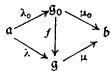
\includegraphics[keepaspectratio]{images/part001_108a7b03.jpg}}

是交换的，因此两个扩张等价。

例 1. 设 g 是 K 上的李代数，D 是 g 的导子。令 h 为交换李代数 K。映射 \(\lambda \mapsto \lambda D (\lambda \in \mathbf{K})\) 是从 h 到 g 的导子李代数的同态。我们构造 h 由 g 作的相应半直积 t。令 \(x_0\) 为 t 的元素 (0, 1)。对所有 \(x \in g\)，有 Dx = [x₀, x]。

例 2. 设 g 是 K 上的李代数，M 是 K-模，\(\rho\) 是从 g 到 gl(M) 的同态。若把 M 视为交换李代数，则 M 的导子李代数就是 gl(M)。因此，我们可以构造对应于 \(\rho\) 的 M 由 g 作的半直积 h。

特别地，令 \(\mathfrak{g} = \mathfrak{gl}(\mathbf{M})\)，\(\rho\) 为 \(\mathfrak{gl}(\mathbf{M})\) 的恒等映射。于是，\(\mathfrak{g}\) 由 \(\mathbf{M}\) 作的半直积记作 \(\mathfrak{af}(\mathbf{M})\)（或记作 \(\mathfrak{af}(n,\mathbf{K})\)，当 \(\mathbf{M} = \mathbf{K}^{n}\) 时）。\(\mathfrak{af}(\mathbf{M})\) 的元素是有序对 \((m,u)\)，其中 \(m\in \mathbf{M}\)、\(u\in \mathfrak{gl}(\mathbf{M})\)；括号定义为

\[
[ (m, u), (m ^ {\prime}, u ^ {\prime}) ] = (u (m ^ {\prime}) - u ^ {\prime} (m), [ u, u ^ {\prime} ]).
\]

*当 M 是 R 上的有限维向量空间时，\(\mathfrak{af}(M)\) 自然地与 M 的仿射群的李代数相同。*

设 \(t\) 是 \(K\) 上的李代数。线性映射 \(\theta\) 从 \(t\) 到 \(\mathfrak{af}(M)\) 可写成 \(x \mapsto ((\zeta(x), \eta(x))\)，其中 \(\zeta\) 是从 \(t\) 到 \(M\) 的线性映射，\(\eta\) 是从 \(t\) 到 \(\mathfrak{gl}(M)\) 的线性映射。我们考察 \(\zeta\) 和 \(\eta\) 为使 \(\theta\) 成为同态必须满足的条件。对 \(x \in t, y \in t\)，必须有

\[
\theta ([ x, y ]) = [ \theta (x), \theta (y) ]
\]

即

\[
\begin{array}{r l} (\zeta ([ x, y ]), \eta ([ x, y ])) & = [ (\zeta (x), \eta (x)), (\zeta (y), \eta (y)) ] \\ & = (\eta (x). \zeta (y) - \eta (y). \zeta (x), [ \eta (x), \eta (y) ]). \end{array}
\]

因此，\(\theta\) 是从 \(t\) 到 \(\mathfrak{af}(M)\) 的同态的充要条件是：\(\eta\) 是从 \(t\) 到 \(\mathfrak{gl}(M)\) 的同态，且 \(\zeta\) 满足关系式：

\[
\zeta ([ x, y ]) = \eta (x). \zeta (y) - \eta (y). \zeta (x).\tag{13}
\]

令 \(\mathbf{N}\) 为 \(\mathbf{K}\)-模 \(\mathbf{M} \times \mathbf{K}\)。取 \(t\) 为 \(\mathfrak{gl}(\mathbf{N})\) 的子代数，由 \(w \in \mathfrak{gl}(\mathbf{N})\) 且满足 \(w(\mathbf{N}) \subset \mathbf{M}\) 的元素组成。对所有 \(w \in t\)，令 \(\eta(w) \in \mathfrak{gl}(\mathbf{M})\) 为 \(w\) 在 \(\mathbf{M}\) 上的限制，并令 \(\zeta(w) = w(0,1) \in \mathbf{M}\)。对 \(w_1 \in t, w_2 \in t\)，

\[
\zeta ([ w _ {1}, w _ {2} ]) = w _ {1} (\zeta (w _ {2})) - w _ {2} (\zeta (w _ {1})) = \eta (w _ {1}). \zeta (w _ {2}) - \eta (w _ {2}). \zeta (w _ {1}).
\]

因此映射 \(w \mapsto (\zeta(w), \eta(w))\) 是同态 \(\theta\)，它从 \(t\) 到 \(\mathfrak{af}(\mathbf{M})\)。显然 \(\theta\) 是双射。令 \(\phi = \theta^{-1}\)。若 \((m, u) \in \mathfrak{af}(\mathbf{M})\)，则 \(\phi(m, u)\) 是元素 \(w\)，它是 \(t\) 中由下式定义的：

\[
w (m ^ {\prime}, \lambda) = (u (m ^ {\prime}) + \lambda m, 0).
\]

\(\mathfrak{af}(\mathbf{M})\) 常被认作子代数 \(\mathfrak{t}\)，它属于 \(\mathfrak{gl}(\mathbf{N})\)，对应的同构为 \(\phi\)。

*当 M 是 \(\mathbf{R}\) 上的有限维向量空间时，同态 \(\phi\) 从 \(\mathfrak{af}(M)\) 到 \(\mathfrak{gl}(N)\)，对应于 M 的仿射群 A 到同态 \(\psi\)，它映到 \(\mathbf{GL}(N)\)；若 \(a \in A\)，则 \(\psi(a)\) 是唯一元素 \(g\)，它属于 \(\mathbf{GL}(N)\) 且满足 \(g(m, 1) = (a(m), 1)\) 对所有 \(m \in M\) 成立。此同态是单射，而 \(\psi(A)\) 是 N 的所有平行于 M 的线性簇均保持不变的自同构组成的集合。*

\subsection{基环变换}

设 \(K_{0}\) 是含单位元的交换环，\(\rho\) 是将单位元映到单位元的从 \(K_{0}\) 到 K 的同态。设 g 是 K 上的李代数。令 \(g'\) 表示将 g 视为 \(K_{0}\) 上的代数并借助 \(\rho\) 得到的代数（参见第 1 号）。则 \(g'\) 是李代数。g 的子代数（分别为理想）是 \(g'\) 的子代数（分别为理想）。若 a 和 b 是 g 的子模，则括号 {[}a, b{]} 在 g 和 \(g'\) 中相同；因为 {[}a, b{]} 是形如

\(\sum_{i=1}^{n}\left[x_i,y_i\right]\) 的元素组成的集合，其中 \(x_{i}\in a,y_{i}\in b\)。由此 \(\mathcal{D}^p\mathfrak{g} = \mathcal{D}^p\mathfrak{g}'\)、\(\mathcal{C}^p\mathfrak{g} = \mathcal{C}^p\mathfrak{g}'\) 对所有 \(p\) 成立。

子集的中心化子在 \(\mathfrak{g}\) 和 \(\mathfrak{g}'\) 中相同。因此 \(\mathcal{C}_p\mathfrak{g} = \mathcal{C}_p\mathfrak{g}'\) 对所有 \(p\) 成立。

设 \(\mathbf{K}_1\) 是含单位元的交换环，\(\sigma\) 是将单位元映到单位元的从 \(\mathbf{K}\) 到 \(\mathbf{K}_1\) 的同态。设 \(\mathfrak{g}\) 是 \(\mathbf{K}\) 上的李代数。令 \(\mathfrak{g}_{(\mathbf{K}_1)}\) 表示 \(\mathbf{K}_1\) 上通过扩张基环由 \(\mathfrak{g}\) 导出的代数（参见第 1 号）。则 \(\mathfrak{g}_{(\mathbf{K}_1)}\) 是李代数。若 \(\mathfrak{a}\) 是 \(\mathfrak{g}\) 的子代数（分别为理想），则 \(\mathfrak{a}_{(\mathbf{K}_1)}\) 在 \(\mathfrak{g}_{(\mathbf{K}_1)}\) 中的典范像是 \(\mathfrak{g}_{(\mathbf{K}_1)}\) 的子代数（分别为理想）。若 \(\mathfrak{a}\) 和 \(\mathfrak{b}\) 是 \(\mathfrak{g}\) 的子模，则 \(\mathfrak{g}_{(\mathbf{K}_1)}\) 中 \([\mathfrak{a},\mathfrak{b}]_{(\mathbf{K}_1)}\) 的典范像，等于 \(\mathfrak{a}_{(\mathbf{K}_1)}\) 和 \(\mathfrak{b}_{(\mathbf{K}_1)}\) 的典范像的括号。由此，\(\mathcal{D}^p (\mathfrak{g}_{(\mathbf{K}_1)})\) 是 \((\mathcal{D}^p\mathfrak{g})_{(\mathbf{K}_1)}\) 的典范像，而 \(\mathcal{C}^p (\mathfrak{g}_{(\mathbf{K}_1)})\) 是 \((\mathcal{C}^p\mathfrak{g})_{(\mathbf{K}_1)}\) 的典范像。

若 K 是域，\(K_{1}\) 是 K 的扩域，\(\sigma\) 是 K 到 \(K_{1}\) 的典范嵌入，则在通常的同一视下有

\[
\begin{array}{c} [ a, b ] _ {(\mathbf {K} _ {1})} = [ a _ {(\mathbf {K} _ {1})}, b _ {(\mathbf {K} _ {1})} ], \qquad \mathcal {D} ^ {p} (\mathfrak {g} _ {(\mathbf {K} _ {1})}) = (\mathcal {D} ^ {p} \mathfrak {g}) _ {(\mathbf {K} _ {1})}, \\ \mathcal {C} ^ {p} (\mathfrak {g} _ {(\mathbf {K} _ {1})}) = (\mathcal {C} ^ {p} \mathfrak {g}) _ {(\mathbf {K} _ {1})}. \end{array}
\]

这些结果将在第 2 节第 9 号中补充完整。

若 M 是域 K 上的有限维向量空间，则 \(M_{(\mathbf{K}_{1})}\) 是 \(K_{1}\) 上的有限维向量空间，结合代数 \(\mathcal{L}(M_{(\mathbf{K}_{1})})\) 自然地与结合代数 \(\mathcal{L}(M)_{(\mathbf{K}_{1})}\) 相同。因此李代数 \(\mathfrak{gl}(M_{(\mathbf{K}_{1})})\) 自然地与李代数 \(\mathfrak{gl}(M)_{(\mathbf{K}_{1})}\) 相同。

\section{李代数的包络代数}

\subsection{包络代数的定义}

设 g 是 K 上的李代数。对于 K 上任意含单位元的结合代数 L，从 g 到 L 的 \(\alpha\)-映射是从 g 到 L 的 K-线性映射 \(\sigma\)，满足

\[
\sigma ([ x, y ]) = \sigma (x) \sigma (y) - \sigma (y) \sigma (x) \quad (x, y \text {   in   } g)
\]

（换言之，是从 \(\mathfrak{g}\) 到与 L 相关联的李代数的同态）。若 L' 是 K 上另一个含单位元的结合代数，\(\tau\) 是将 1 映到 1 的从 L 到 L' 的同态，则 \(\tau \circ \sigma\) 是一个 \(\alpha\)-映射，从 \(\mathfrak{g}\) 到 L'。我们要寻找一个含单位元的结合代数以及一个 \(\alpha\)-映射，从 \(\mathfrak{g}\) 到该代数，二者具有泛性质（Set Theory, Chapter IV, § 3, no. 1）。

定义 1. 设 \(\mathfrak{g}\) 是 \(\mathbf{K}\) 上的李代数，\(\mathbf{T}\) 是 \(\mathbf{K}\)-模 \(\mathfrak{g}\) 的张量代数，\(\mathbf{J}\) 是 \(\mathbf{T}\) 的双边理想，由张量 \(x \otimes y - y \otimes x - [x, y]\)（其中 \(x \in \mathfrak{g}, y \in \mathfrak{g}\)）生成。结合代数 \(\mathbf{U} = \mathbf{T} / \mathbf{J}\) 称为 \(\mathfrak{g}\) 的包络代数。在 \(\mathfrak{g}\) 上，将 \(\mathbf{T}\) 映到 \(\mathbf{U}\) 的典范映射的限制称为从 \(\mathfrak{g}\) 到 \(\mathbf{U}\) 的典范映射。

令 \(T_{+}\) 为 T 的双边理想，由 0 阶分量为零的张量组成。令 \(\mathrm{T}_0 = \mathrm{K}.1\) 为 T 中 0 阶元素的集合。令 \(\mathrm{U}_{+}\) 和 \(\mathrm{U}_0\) 为 \(\mathrm{T}_{+}\) 和 \(\mathrm{T}_0\) 在 U 中的典范像。由于 \(\mathrm{J} \subset \mathrm{T}_{+}\)，直和分解 \(\mathrm{T} = \mathrm{T}_0 + \mathrm{T}_{+}\) 蕴含直和分解 \(\mathrm{U} = \mathrm{U}_0 + \mathrm{U}_{+}\)。因此代数 U 有一个异于 0 的单位元，且 \(\mathrm{U}_0 = \mathrm{K}.1\)。对所有 \(x \in \mathbf{U}\)，\(x\) 在 \(\mathrm{U}_0\) 中的分量称为 \(x\) 的常数项。常数项为零的元素构成 U 的双边理想，即由 g 在 U 中的典范像生成的双边理想 \(\mathrm{U}^{+}\)。

结合代数 U 由 1 和 g 在 U 中的典范像生成。

若 \(x \in \mathfrak{g}\) 且 \(y \in \mathfrak{g}\)，则 \(x \otimes y - y \otimes x\) 与 \([x, y]\) 在 T 中模 J 同余；因此，若 \(\sigma_0\) 表示从 \(\mathfrak{g}\) 到 U 的典范映射，则

\[
\sigma_ {0} (x) \sigma_ {0} (y) - \sigma_ {0} (y) \sigma_ {0} (x) = \sigma_ {0} ([ x, y ])
\]

在 U 中成立。换言之，\(\sigma_{0}\) 是从 g 到 U 的 \(\alpha\)-映射。

命题 1. 设 \(\sigma\) 是一个 \(\alpha\)-映射，从 \(\mathfrak{g}\) 到含单位元的结合代数 \(\mathbf{L}\)。存在唯一的同态 \(\tau\)，它从 \(\mathbf{U}\) 到 \(\mathbf{L}\)，将 1 映到 1，且满足 \(\sigma = \tau \circ \sigma_0\)，其中 \(\sigma_0\) 表示从 \(\mathfrak{g}\) 到 \(\mathbf{U}\) 的典范映射。

设 \(\tau'\) 是从 T 到 L 的唯一同态，它延拓 \(\sigma\) 并将 1 映到 1。则对 g 中的 \(x, y\)，

\[
\tau^ {\prime} (x \otimes y - y \otimes x - [ x, y ]) = \sigma (x) \sigma (y) - \sigma (y) \sigma (x) - \sigma ([ x, y ]) = 0;
\]

故 \(\tau'\) 在 \(J\) 上为零，取商后定义了同态 \(\tau\)，它从 \(U\) 到 \(L\)，将 1 映到 1，并满足 \(\sigma = \tau \circ \sigma_0\)。由于 \(\tau\) 由 \(\sigma_0(g)\) 和 1 在代数 \(U\) 中生成，其唯一性是显然的。

设 \(g'\) 是 K 上的另一个李代数，U' 是其包络代数，\(\sigma_0'\) 是从 \(g'\) 到 U' 的典范映射。设 \(\phi\) 是从 g 到 g' 的同态。则 \(\sigma_0' \circ \phi\) 是从 g 到 U' 的 \(\alpha\)-映射；因此存在唯一的将 1 映到 1 的从 U 到 U' 的同态 \(\tilde{\phi}\)，使下图

\[
\begin{array}{c} g \xrightarrow {\phi} g ^ {\prime} \\ \sigma_ {0} \Biggl \downarrow \\ U \xrightarrow {\tilde {\phi}} U ^ {\prime} \end{array}
\]

是交换的。此同态将 U 中常数项为零的元素映到 U' 中常数项为零的元素。若 g'' 是 K 上的另一个李代数，\(\phi'\) 是从 g' 到 g'' 的同态，则 \(\widetilde{\phi'\circ\phi}=\widetilde{\phi}'\circ\widetilde{\phi}\)。

\subsection{李代数积的包络代数}

设 \(g_{1}, g_{2}\) 是 K 上的两个李代数，\(U_{i}\) 是 \(g_{i}\) 的包络代数，\(\sigma_{i}\) 是从 \(g_{i}\) 到 \(U_{i}\) 的典范映射（i = 1, 2）。令 \(g = g_{1} \times g_{2}\)，U 为其包络代数，\(\sigma\) 为从 g 到 U 的典范映射。\(g_{1}\) 和 \(g_{2}\) 到 g 的典范嵌入定义了从 \(U_{1}\) 和 \(U_{2}\) 到 U 的典范同态；它们的像彼此可交换，因而得到同态 \(\phi\)，它从代数 \(U_1 \otimes_K U_2\) 到代数 \(U\)，并将 1 映到 1。

命题 2. 同态 \(\phi\) 是代数同构

映射 \(\sigma': (x_1, x_2) \mapsto \sigma_1(x_1) \otimes 1 + 1 \otimes \sigma_2(x_2) (x_1 \in \mathfrak{g}_1, x_2 \in \mathfrak{g}_2)\) 是一个 \(\alpha\)-映射，从 \(\mathfrak{g}\) 到 \(\mathrm{U}_1 \otimes_{\mathbb{K}} \mathrm{U}_2\)，因此存在唯一的同态 \(\tau\)，它从 \(\mathrm{U}\) 到 \(\mathrm{U}_1 \otimes_{\mathbb{K}} \mathrm{U}_2\)，将 1 映到 1（第 1 号，命题 1），使得：

\[
\sigma^ {\prime} = \tau \circ \sigma .\tag{1}
\]

现在 \(\phi \circ \tau \circ \sigma = \phi \circ \sigma' = \sigma\)，且 \(\tau \circ \phi \circ \sigma' = \tau \circ \sigma = \sigma'\)，所以 \(\phi \circ \tau\) 和 \(\tau \circ \phi\) 分别是 U 与 \(U_1 \otimes_K U_2\) 的恒等映射。故命题得证。

\(U_{1} \otimes_{K} U_{2}\) 在同构 \(\phi\) 下与 U 相同。于是 g 到 U 的典范映射由 (1) 与下列映射相同：

\[
(x _ {1}, x _ {2}) \mapsto \sigma_ {1} (x _ {1}) \otimes 1 + 1 \otimes \sigma_ {2} (x _ {2}).
\]

类似地，若 \(g_{1},\ldots,g_{n}\) 是 K 上的李代数，其包络代数为 \(U_{1},\ldots,U_{n}\)，则 \(g_{1}\times\cdots\times g_{n}\) 的包络代数 U 自然地与 \(U_{1}\otimes_{K}\cdots\otimes_{K}U_{n}\) 相同，而 \(g_{1}\times\cdots\times g_{n}\) 到 U 的典范映射与下列映射相同：

\[
(x _ {1}, \dots , x _ {n}) \mapsto \sigma_ {1} (x _ {1}) \otimes 1 \otimes \dots \otimes 1 + \dots + 1 \otimes \dots \otimes 1 \otimes \sigma_ {n} (x _ {n})
\]

（\((\sigma_{i} \text{ 所表示的典范映射从 } g_{i} \text{ 到 } U_{i})\)）。

\subsection{李子代数的包络代数}

设 g 是 K 上的李代数，h 是 g 的子代数，\(\sigma\)、\(\sigma'\) 分别是 g、h 到其包络代数 U、V 的典范映射。于是 h 到 g 的典范嵌入 i 定义了一个从 V 到 U 的同态 i，称为典范同态，并满足 \(\sigma \circ i = i \circ \sigma'\)。代数 \(i(\mathrm{V})\) 由 1 和 \(\sigma(\mathfrak{h})\) 生成。我们将看到（第 7 号，定理 5 的推论），在重要的情形中 i 是单射。

若 \(\mathfrak{h}\) 是 \(\mathfrak{g}\) 的理想，则由 \(\sigma(\mathfrak{h})\) 生成的 U 的左理想与由 \(\sigma(\mathfrak{h})\) 生成的右理想相同，换言之，它是双边理想 R。这是因为对 \(x \in \mathfrak{h}\) 和 \(x' \in \mathfrak{g}\)，

\[
\sigma (x) \sigma (x ^ {\prime}) = \sigma (x ^ {\prime}) \sigma (x) + \sigma ([ x, x ^ {\prime} ])
\]

且 \([x, x'] \in \mathfrak{h}\)。

命题 3. 设 \(\mathfrak{h}\) 是一个理想，并令 \(\mathfrak{g}, p\) 分别表示一个李代数及其典范满同态；该同态从 \(\mathfrak{g}\) 到 \(\mathfrak{g} / \mathfrak{h}\)，W 是 \(\mathfrak{g} / \mathfrak{h}\) 的包络代数。同态：

\[
\tilde {p}: \mathrm{U} \rightarrow \mathrm{W}
\]

由 \(p\) 典范定义的映射是满射，其核是理想 \(R\)，位于 \(U\) 中，并由 \(\sigma(h)\) 生成。

令 \(\sigma''\) 为从 \(g/h\) 到 W 的典范映射。交换图：

\pandocbounded{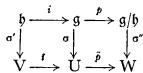
\includegraphics[keepaspectratio]{images/part001_4ab4ddcc.jpg}}

表明 \(\tilde{p}\) 在 \(\sigma(\mathfrak{h})\) 上为零，从而在 R 上为零。令 \(\psi\) 为从 U 到 U/R 的典范满同态。存在从 U/R 到 W 的同态 \(\phi\)

\pandocbounded{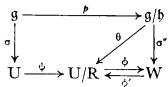
\includegraphics[keepaspectratio]{images/part001_c6a5c19d.jpg}}

到 W，使 \(\tilde{p} = \phi \circ \psi\)。映射 \(\psi \circ \sigma\) 把 \(g\) 映到 U/R，是一个 \(\alpha\)-映射，并且在 \(h\) 上为零，因而定义了一个 \(\alpha\)-映射 \(\theta\)，从 \(g / h\) 到 U/R，满足 \(\theta \circ p = \psi \circ \sigma\)。于是 \(\phi \circ \theta \circ p = \phi \circ \psi \circ \sigma = \sigma'' \circ p\)，所以 \(\phi \circ \theta = \sigma''\)。存在唯一的将 1 映到 1 的从 W 到 U/R 的同态 \(\phi'\)（第 1 号，命题 1），使 \(\theta = \phi' \circ \sigma''\)。于是 \(\phi' \circ \phi \circ \theta = \phi' \circ \sigma'' = \theta\)，且 \(\phi \circ \phi' \circ \sigma'' = \phi \circ \theta = \sigma''\)，因此 \(\phi' \circ \phi\) 和 \(\phi \circ \phi'\) 分别是 U/R 和 W 的恒等映射。证毕。

U/R 在同构 \(\phi\) 下与 W 相同。于是典范映射 \(\sigma''\) 将 \(g/h\) 映到 W，并与 \(\theta\) 相同，也就是与由取商后得到的将 \(g/h\) 映到 U/R 的映射 \(\sigma\) 相同。

\subsection{逆李代数的包络代数}

设 \(g\) 是 \(K\) 上的李代数，\(g^0\) 是逆李代数，\(\sigma\) 和 \(\sigma_0\) 分别是将 \(g\) 和 \(g^0\) 映到其包络代数 \(U\) 和 \(V\) 的典范映射。则 \(\sigma\) 是一个 \(\alpha\)-映射，从 \(g^0\) 到结合代数 \(U^0\)，即结合代数 \(U\) 的逆代数。因此存在唯一的同态 \(\phi\)，它从 \(V\) 到 \(U^0\)，将 1 映到 1，并满足 \(\sigma = \phi \circ \sigma_0\)。

命题 4. 同态 \(\phi\) 是从 \(V\) 到 \(U^0\) 的同构。

存在同态 \(\phi'\)，它将 U 映到 \(V^0\)，将 1 映到 1，并满足 \(\sigma_0 = \phi' \circ \sigma\)。可将 \(\phi'\) 视为从 \(U^0\) 到 V 的同态。于是 \(\sigma_0 = \phi' \circ \phi \circ \sigma_0\)，且 \(\sigma = \phi \circ \phi' \circ \sigma\)，从而 \(\phi' \circ \phi\) 和 \(\phi \circ \phi'\) 分别是 V 和 U 的恒等映射。故命题得证。

V 与 \(U^{0}\) 相同，这一识别由同构 \(\phi\) 给出。于是 \(\sigma_{0}\) 与 \(\sigma\) 相同。

在此同一视下，同构 \(\theta: x \mapsto -x\) 从 \(\mathfrak{g}\) 到 \(\mathfrak{g}^0\)，定义了同构 \(\tilde{\theta}\) 从 U 到 V = U \(^0\)。此同构可视为 U 的反自同构，称为 U 的主反自同构。若 \(x_{1}, \ldots, x_{n}\) 属于 \(\mathfrak{g}\)，则：

\[
\begin{array}{r l} \tilde {\theta} (\sigma (x _ {1}) \dots \sigma (x _ {n})) & = \tilde {\theta} (\sigma (x _ {n})) \dots \tilde {\theta} (\sigma (x _ {1})) = (- \sigma (x _ {n})) \dots (- \sigma (x _ {1})) \\ & = (- 1) ^ {n} \sigma (x _ {n}) \dots \sigma (x _ {1}). \end{array}\tag{2}
\]

\subsection{模的对称代数}

设 V 是 K-模。V 可唯一地视为交换李代数。于是 V 的包络代数可如下得到：令 T 为 V 的张量代数；令 I 为由张量 \(x \otimes y - y \otimes x\)（\(x \in V, y \in V\)）生成的 T 的双边理想；然后构造代数 S = T/I。

回顾 S 被称为 V 的对称代数（Algebra, Chapter III, § 6），我们简要总结本章所需的性质，其证明都是直接的。令 \(T^{n}\) 为 T 中 n 阶齐次张量的集合。则 \(\mathrm{I} = (\mathrm{I} \cap \mathrm{T}^{2}) + (\mathrm{I} \cap \mathrm{T}^{3}) + \cdots\)，从而 S 是各 \(S^{n}\)（它们是 \(T^{n}\) 的典范像）的直和。\(S^{n}\) 的元素称为 n 次齐次元素。\(S^{0} = K.1\)，\(S^{1}\) 与 V 相同，且 \(S^{n}S^{p} \subset S^{n+p}\)。代数 S 由 1 和 \(S^{1} = V\) 生成。显然 \(S^{1}\) 中任意两个元素都可交换，因而 S 是交换的。若 V 是以 \((x_{\lambda})_{\lambda \in \Lambda}\) 为基的自由 K-模，则从多项式代数 \(K[X_{\lambda}]_{\lambda \in \Lambda}\) 到 S 的典范满同态 f（将 1 映到 1，并将 \(X_{\lambda}\) 映到 \(x_{\lambda}\)，对所有 \(\lambda \in \Lambda\)）是同构：因为由 S 的泛性质（第 1 号，命题 1），存在从 S 到 \(K[X_{\lambda}]_{\lambda \in \Lambda}\) 的同态 g，将 1 映到 1，并将 \(x_{\lambda}\) 映到 \(X_{\lambda}\)，对所有 \(\lambda \in \Lambda\)，且 f 与 g 互为逆同态。

令 \(S'^{n} \subset T^n\) 为阶数 \(n\) 的齐次对称张量的集合（Algebra, Chapter III, § 5, no. 1, Definition 2）。若 \(K\) 是特征为 0 的域，则 \(S'^{n}\) 与 \(I \cap T^n\) 在 \(T^n\) 中互为补空间。事实上，设 \((x_{\lambda})_{\lambda \in \Lambda}\) 是 \(V\) 的一个基。给 \(\Lambda\) 赋予全序（Set Theory, Chapter III, § 2, no. 3, Theorem 1）。令 \(\Lambda_n\) 为由 \(n\) 个 \(\Lambda\) 中元素组成的递增序列的集合。对 \(M = (\lambda_1, \ldots, \lambda_n) \in \Lambda_n\)，令

\[
y _ {\mathrm{M}} = \frac {1}{n !} \sum_ {\sigma \in \mathfrak {S} _ {n}} x _ {\lambda_ {\sigma (1)}} \otimes \dots \otimes x _ {\lambda_ {\sigma (n)}}.
\]

\(y_{\mathbf{M}}\) 对于 \(\mathbf{M} \in \Lambda_n\) 构成向量 K-空间 \(\mathbf{S}'^n\) 的一组生成元。根据上段，它们在 \(\mathbf{S}^n\) 中的典范像构成 \(\mathbf{S}^n\) 的一个基。因此 \((y_{\mathbf{M}})_{\mathbf{M} \in \Lambda_n}\) 是 \(\mathbf{I} \cap \mathbf{T}^n\) 在 \(\mathbf{T}^n\) 中的一个补子空间的基（Algebra, Chapter II, § 1, no. 6, Proposition 4），这就证明了断言。

因此，当 K 是特征为 0 的域时，\(S'^{n}\) 上的典范映射 \(T^{n} \rightarrow S^{n}\) 的限制是从空间 \(S'^{n}\) 到空间 \(S^{n}\) 的同构，因而有逆同构。对每个 n 得到的这些逆同构定义了从空间 S 到对称张量空间 \(S' = \sum_{n \geqslant 0} S'^{n}\) 的典范同构。

\subsection{包络代数的滤子}

设 g 是 K 上的李代数，T 是 K-模 g 的张量代数。令 \(T^{n}\) 为 T 中由 n 阶齐次张量组成的子模

并令 \(\mathrm{T_n} = \sum_{i\leqslant n}\mathrm{T^i}\)。则 \(\mathrm{T_n}\subset \mathrm{T}_{n + 1},\mathrm{T_0} = \mathrm{K}.1,\mathrm{T}_{-1} = \{0\}\)，且 \(\mathrm{T_nT_p}\subset \mathrm{T}_{n + p}\)。令 \(\mathbf{U}_n\) 为 \(\mathbf{T}_n\) 在 g 的包络代数 U 中的典范像。则 \(\mathrm{U_n}\subset \mathrm{U}_{n + 1},\mathrm{U_0} = \mathrm{K}.1,\mathrm{U}_{-1} = \{0\}\)，且 \(\mathrm{U_nU_p}\subset \mathrm{U}_{n + p}\)；因此 U 可描述为由 \(\mathbf{U}_n\) 滤过的代数（Commutative Algebra, Chapter III, §2, no. I）；\(\mathrm{U_n}\) 中的元素称为滤子次数 \(\leqslant n\) 的元素。

令 \(G^n\) 为 K-模 \(U_n / U_{n-1}\)，令 G 为各 \(G^n\) 的直和这个 K-模。U 上的乘法在取商后定义了从 \(G^n \times G^m\) 到 \(G^{n+m}\) 的双线性映射，因而定义了从 \(G \times G\) 到 G 的双线性映射，该映射是结合的。于是 G 具有结合 K-代数结构。并且 \(G^n G^m \subset G^{n+m}\)。\(G^n\) 的元素称为 n 次元素。如此得到的分次代数正是滤过代数 U 的关联分次代数（Commutative Algebra, Chapter III, § 2, no. 3）。

令 \(\phi_{n}\) 为下列典范 K-线性映射的复合

\[
\mathrm{T} ^ {n} \rightarrow \mathrm{U} _ {n} \rightarrow \mathrm{G} ^ {n}.
\]

由于 \(\mathbf{T}^n\) 是 \(\mathbf{T}_{n - 1}\) 在 \(\mathbf{T}_n\) 中的补空间，\(\phi_n\) 是满射。各 \(\phi_n\) 定义了 K-线性满射 \(\phi\)，它从 \(\sum_{n}\mathbf{T}^{n} = \mathbf{T}\) 到 \(\sum_{n}\mathbf{G}^{n} = \mathbf{G}\)。

命题 5. 从 T 到 G 的映射 \(\phi\) 是将 1 映到 1 的代数同态，并且在由张量 \(x \otimes y - y \otimes x\)（\(x \in \mathfrak{g}, y \in \mathfrak{g}\)）生成的双边理想上为零。

若 \(t \in \mathbf{T}^n\) 且 \(t' \in \mathbf{T}^p\)，则按乘法定义，有 \(\phi(t)\phi(t') = \phi(tt')\)，其中乘法定义在 \(\mathbf{G}\) 上。所以 \(\phi\) 是代数同态，且显然 \(\phi(1) = 1\)。若 \(x, y\) 属于 \(\mathfrak{g}\)，则 \(x \otimes y - y \otimes x \in \mathbf{T}^2\)，且此元素在 \(\mathrm{U}_2\) 中的典范像等于 \([x, y]\) 的典范像，因而属于 \(\mathrm{U}_1\)。所以 \(\phi(x \otimes y - y \otimes x) = 0\)，命题得证。

令 S 为 K-模 g 的对称代数，\(\tau\) 为从 T 到 S 的典范同态。命题 5 表明，存在唯一的将 1 映到 1 的从代数 S 到代数 G 的同态 \(\omega\)，称为典范同态，使 \(\phi = \omega \circ \tau\)。有 \(\omega(\mathrm{S}^{n}) = \phi(\mathrm{T}^{n}) = \mathrm{G}^{n}\)。令 \(\tau_{n}\) 为 \(\tau\) 在 \(T^{n}\) 上的限制，\(\omega_{n}\) 为 \(\omega\) 在 \(S^{n}\) 上的限制，\(\psi_{n}\) 为从 \(T^{n}\) 到 \(U_{n}\) 的典范映射，\(\theta_{n}\) 为从 \(U_{n}\) 到 \(G^{n}\) 的典范映射。由 \(\omega_{n}\) 的定义，下图交换：

\pandocbounded{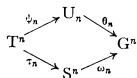
\includegraphics[keepaspectratio]{images/part001_82008693.jpg}}

命题 6. 若 K 是 Noetherian 环且 g 是有限生成模，则环 U 是左、右 Noetherian 的。

S 是 K 上的有限生成代数，因而是 Noetherian 环（Commutative Algebra, Chapter III, § 2, no. 10, Corollary 3 to Theorem 2）。所以，与 S 的商环同构的 G 是 Noetherian 的。因此 U 是左、右 Noetherian 的（Commutative Algebra, Chapter III, § 2, no. 10, Remark 2）。

推论. 设 K 是域，g 是 K 上的有限维空间。令 \(I_{1}, \ldots, I_{m}\) 为 U 中有限余维的右（分别为左）理想。则积理想 \(I_{1}I_{2}\ldots I_{m}\) 具有有限余维。

对 m 归纳，只需考虑例如两个右理想的情形。右 U-模 \(I_{1}\) 由有限个元素 \(u_{1},\ldots,u_{p}\) 生成（命题 6）。令 \(v_{1},\ldots,v_{q}\) 为 U 中的元素，使其模 \(I_{2}\) 的类生成向量空间 \(U/I_{2}\)。于是，\(I_{1}/I_{1}I_{2}\) 中 \(u_{i}v_{j}\) 的典范像生成向量空间 \(I_{1}/I_{1}I_{2}\)，该空间因而是有限维的。所以 \(\dim_{\mathbb{K}}(\mathrm{U}/\mathrm{I}_{1}\mathrm{I}_{2})=\dim_{\mathbb{K}}(\mathrm{U}/\mathrm{I}_{1})+\dim_{\mathbb{K}}(\mathrm{I}_{1}/\mathrm{I}_{1}\mathrm{I}_{2})<+\infty\)。

注. 设 \(g'\) 是环 K 上的另一个李代数，\(U'\) 是其包络代数，\(U_n'\) 是 \(U'\) 中滤子次数 \(\leqslant n\) 的元素的集合，\(U^n\)（分别为 \(U'^n\)）是 U（分别为 \(U'\)）中 g（分别为 \(g'\)）的 n 阶齐次对称张量的典范像的集合。令 \(\eta\) 为从 g 到 \(g'\) 的同态，\(\tilde{\eta}\) 为相应的从 U 到 \(U'\) 的同态。则

\[
\tilde {\eta} (\mathrm{U} _ {n}) \subset \mathrm{U} _ {n} ^ {\prime}, \quad \tilde {\eta} (\mathrm{U} ^ {n}) \subset \mathrm{U} ^ {\prime n}.
\]

特别地，U 的主反自同构保持 \(U_{n}\) 和 \(U^{n}\) 稳定。将 \(T^{n}\) 映到自身的 K-线性映射为：

\[
x _ {1} \otimes x _ {2} \otimes \dots \otimes x _ {n} \quad \text { to } \quad x _ {n} \otimes x _ {n - 1} \otimes \dots \otimes x _ {1}
\]

对 g 中所有 \(x_{1},\ldots,x_{n}\) 的映射是一个对称算子，因而保持 n 阶齐次对称张量不变。因此，U 的主反自同构在每个 \(U^{n}\) 上诱导出比为 \((-1)^{n}\) 的伸缩变换。

\subsection{Poincaré-Birkhoff-Witt 定理}

定理 1. 设 \(\mathfrak{g}\) 是李 K-代数，\(U\) 是其包络代数，G 是滤过代数 U 的关联分次代数，S 是 K-模 \(\mathfrak{g}\) 的对称代数。若 \(\mathfrak{g}\) 是自由 K-模，则典范同态 \(\omega: \mathrm{S} \to \mathrm{G}\) 是同构。

令 \((x_{\lambda})_{\lambda \in \Lambda}\) 为 K-模 g 的一个基；给 \(\Lambda\) 赋予全序（Set Theory, Chapter III, § 2, no. 3, Theorem 1）。令 P 为多项式代数 \(\mathrm{K}[z_{\lambda}]_{\lambda \in \Lambda}\)，其不定元 \(z_{\lambda}\) 与 \(x_{\lambda}\) 一一对应。对于 \(\mathrm{M} = (\lambda_1, \lambda_2, \ldots, \lambda_n)\) 中元素组成的每个序列 \(\Lambda\)，令 \(z_{\mathrm{M}}\) 表示单项式 \(z_{\lambda_1}z_{\lambda_2}\ldots z_{\lambda_n}\)，令 \(x_{\mathrm{M}}\) 表示张量 \(x_{\lambda_1}\otimes x_{\lambda_2}\otimes \dots \otimes x_{\lambda_n}\)。

当  递增时，\(z_{\mathbb{M}}\) 构成 K-模 \(\mathbf{M}\)\(\mathbf{P}\) 的一个基（约定 \(\varnothing\) 是递增序列，且 \(z_{\varnothing} = 1\)）。令 \(\mathbf{P}_p\) 为次数 \(\leqslant p\) 的多项式组成的子模。我们先证明若干引理。（为简便起见，若对序列 M 的每个指标  都有 ，就写作 \(\lambda \leqslant M\)\(\lambda \leqslant \mu\)\(\mu\)。）

引理 1. 对每个整数 \(p \geqslant 0\)，存在唯一的从 K-模 \(f_p\)\(\mathfrak{g} \otimes_{\mathbb{K}} \mathrm{P}_p\) 到 K-模 \(\mathrm{P}\) 的同态 ，满足下列条件：

\[
\left(\mathrm{A} _ {p}\right) \quad f _ {p} \left(x _ {\lambda} \otimes z _ {\mathrm{M}}\right) = z _ {\lambda} z _ {\mathrm{M}} \quad \text {   for   } \lambda \leqslant \mathrm{M}, z _ {\mathrm{M}} \in \mathrm{P} _ {p};
\]

\[
\left(\mathrm{B} _ {p}\right) \quad f _ {p} \left(x _ {\lambda} \otimes z _ {\mathrm{M}}\right) - z _ {\lambda} z _ {\mathrm{M}} \in \mathrm{P} _ {q} \quad for \quad z _ {\mathrm{M}} \in \mathrm{P} _ {q}, q \leqslant p;
\]

\[
\left(\mathrm{C} _ {p}\right) \quad f _ {p} \left(x _ {\lambda} \otimes f _ {p} \left(x _ {\mu} \otimes z _ {\mathrm{N}}\right)\right) = f _ {p} \left(x _ {\mu} \otimes f _ {p} \left(x _ {\lambda} \otimes z _ {\mathrm{N}}\right)\right) + f _ {p} \left(\left[ x _ {\lambda}, x _ {\mu} \right] \otimes z _ {\mathrm{N}}\right)
\]

对 \(z_{\mathbf{N}} \in \mathbf{P}_{p-1}\) 成立。（\((\mathbf{C}_p)\) 中出现的各项由 \((\mathbf{B}_p)\) 可知有意义。）

此外，\(f_{p}\) 在 \(\mathfrak{g} \otimes \mathrm{P}_{p-1}\) 上的限制与 \(f_{p-1}\) 一致。

最后一个断言由其余断言推出，因为 \(f_{p}\) 在 \(\mathfrak{g} \otimes_{\mathbb{K}} \mathrm{P}_{p-1}\) 上的限制满足条件 \((\mathrm{A}_{p-1})\)、\((\mathrm{B}_{p-1})\) 和 \((\mathrm{C}_{p-1})\)。我们对 p 归纳证明 \(f_{p}\) 的存在性和唯一性。当 \(p\)\(p = 0\) 时，条件 \((\mathrm{A}_0)\) 给出 \(f_0(x_\lambda \otimes 1) = z_\lambda\)，此时条件 \((\mathrm{B}_0)\) 和 \((\mathrm{C}_0)\) 显然满足。现在假设 \(f_{p-1}\) 的存在性和唯一性已经证明。我们说明，\(f_{p-1}\) 有唯一延拓 \(f_{p}\) 到 \(\mathfrak{g} \otimes_{\mathbb{K}} \mathrm{P}_{p}\)，并满足条件 \((\mathrm{A}_{p})\)、\((\mathrm{B}_{p})\) 和 \((\mathrm{C}_{p})\)。

对于含 p 个元素的递增序列 M，我们必须定义 \(f_{p}(x_{\lambda} \otimes z_{\mathbb{M}})\)。

若 \(\lambda \leqslant M\)，其值由条件 \((A_p)\) 给出。否则，M 可唯一写成 \(M\)\((\mu, N)\) 的形式，其中 \(\mu < \lambda\)、\(\mu \leqslant N\)。于是

\[
z _ {\mathrm{M}} = z _ {\mu} z _ {\mathrm{N}} = f _ {p - 1} (x _ {\mu} \otimes z _ {\mathrm{N}})
\]

由 \((\mathrm{A}_{p - 1})\)，所以 \((\mathrm{C}_p)\) 的左端就是 \(f_{p}(x_{\lambda}\otimes z_{\mathbb{M}})\)。现在 \((\mathrm{C}_p)\) 的右端已经定义好：根据 \((\mathrm{B}_{p - 1})\)，可写为：

\[
f _ {p} (x _ {\lambda} \otimes z _ {\mathrm{N}}) = f _ {p - 1} (x _ {\lambda} \otimes z _ {\mathrm{N}}) = z _ {\lambda} z _ {\mathrm{N}} + w
\]

其中 \(w \in \mathbf{P}_{p-1}\)；因此 \((\mathbf{C}_p)\) 的右端变为：

\[
z _ {\lambda} z _ {\mu} z _ {N} + f _ {p - 1} (x _ {\mu} \otimes w) + f _ {p - 1} ([ x _ {\lambda}, x _ {\mu} ] \otimes z _ {N}).
\]

这样便唯一确定了 \(f_{p}\)，且显然满足条件 \((\mathbf{A}_{p})\) 和 \((\mathbf{B}_{p})\)。当 \((\mathbf{C}_{p})\)\(\mu < \lambda\)、\(\mu \leqslant N\) 时，条件  成立。由于 \([x_{\mu}, x_{\lambda}] = -[x_{\lambda}, x_{\mu}]\)，当 \((\mathbf{C}_{p})\)\(\lambda < \mu\)、\(\lambda \leqslant N\) 时，条件 \((\mathbf{C}_{p})\) 也成立。当 \(\lambda = \mu\) 时 \((\mathbf{C}_{p})\) 显然成立，所以只要 \(\lambda \leqslant N\) 或 \(\mu \leqslant N\)， 就成立。若这些不等式均不成立，则 \(N = (\nu, Q)\)，其中 \(\nu \leqslant Q\)、\(\nu < \lambda\)、\(\nu < \mu\)。以下简写 \(f_{p}(x \otimes z) = xz\)（其中 \(x \in g\)、\(z \in P_{p}\)），由归纳假设有：

\[
x _ {\mu} z _ {N} = x _ {\mu} (x _ {\nu} z _ {Q}) = x _ {\nu} (x _ {\mu} z _ {Q}) + [ x _ {\mu}, x _ {\nu} ] z _ {Q}.
\]

现在 \(x_{\mu}z_{\mathbf{Q}}\) 具有 \(z_{\mu}z_{\mathbf{Q}} + w\) 的形式，其中 \(w\in \mathrm{P}_{p - 2}\)。由于  且 ，可将 (C \(_{p}\) ) 应用于 \(x_{\lambda}(x_{\nu}(z_{\mu}z_{\mathbf{Q}}))\)；根据归纳假设，也可应用于 \(\nu \leqslant Q\)\(\nu < \mu\)\(x_{\lambda}(x_{\nu}w)\)，因而可应用于 \(x_{\lambda}(x_{\nu}(x_{\mu}z_{\mathbf{Q}}))\)。因此：

\[
\begin{array}{r l} x _ {\lambda} (x _ {\mu} z _ {N}) = x _ {\nu} (x _ {\lambda} (x _ {\mu} z _ {\mathbb {Q}})) & + [ x _ {\lambda}, x _ {\nu} ] (x _ {\mu} z _ {\mathbb {Q}}) + [ x _ {\mu}, x _ {\nu} ] (x _ {\lambda} z _ {\mathbb {Q}}) \\ & + [ x _ {\lambda}, [ x _ {\mu}, x _ {\nu} ] ] z _ {\mathbb {Q}}. \end{array}
\]

交换 \(\lambda\) 与 \(\mu\) 后相减：

\[
\begin{array}{r l} {x _ {\lambda} (x _ {\mu} z _ {N}) - x _ {\mu} (x _ {\lambda} z _ {N})} & {= x _ {\nu} (x _ {\lambda} (x _ {\mu} z _ {Q}) - x _ {\mu} (x _ {\lambda} z _ {Q}))} \\ & {\quad + [ x _ {\lambda}, [ x _ {\mu}, x _ {\nu} ] ] z _ {Q} - [ x _ {\mu}, [ x _ {\lambda}, x _ {\nu} ] ] z _ {Q}} \\ & {= x _ {\nu} ([ x _ {\lambda}, x _ {\mu} ] z _ {Q}) + [ x _ {\lambda}, [ x _ {\mu}, x _ {\nu} ] ] z _ {Q} + [ x _ {\mu}, [ x _ {\nu}, x _ {\lambda} ] ] z _ {Q}} \\ & {= [ x _ {\lambda}, x _ {\mu} ] (x _ {\nu} z _ {Q}) + ([ x _ {\nu}, [ x _ {\lambda}, x _ {\mu} ] ]} \\ & {\quad + [ x _ {\lambda}, [ x _ {\mu}, x _ {\nu} ] ] + [ x _ {\mu}, [ x _ {\nu}, x _ {\lambda} ] ]) z _ {Q}} \end{array}
\]

从而由 Jacobi 恒等式

\[
x _ {\lambda} (x _ {\mu} z _ {N}) - x _ {\mu} (x _ {\lambda} z _ {N}) = [ x _ {\lambda}, x _ {\mu} ] z _ {N}
\]

这就完成了引理 1 的证明。

引理 2. 存在从  到  的 \(\alpha\)-映射 \(\sigma\)\(\mathfrak{g}\)\(\mathcal{L}_{\mathbf{K}}(\mathbf{P})\)，使得：

\begin{enumerate}
\def\labelenumi{(\arabic{enumi})}
\item
  \(\sigma(x_{\lambda})z_{\mathbf{M}} = z_{\lambda}z_{\mathbf{M}}\) 对 \(\lambda \leqslant \mathbf{M}\) 成立；
\item
  \(\sigma(x_{\lambda})z_{\mathbf{M}} \equiv z_{\lambda}z_{\mathbf{M}} (\mathrm{mod.~P}_{p})\) 若 \(\mathbf{M}\) 含有 \(p\) 个元素。
\end{enumerate}

由引理 1，对所有 p，存在从 K-模  到 P 的同态 \(f\)，满足条件 \(\mathfrak{g} \otimes_{\mathbb{K}} \mathrm{P}_p\)\(p\)\((\mathrm{A}_p), (\mathrm{B}_p), (\mathrm{C}_p)\)（以 f 替代 \(f_p\)）。此同态定义了从 K-模 \(f\)\(\sigma\)\(\mathfrak{g}\) 到 K-模 \(\mathcal{L}_{\mathbb{K}}(\mathrm{P})\) 的同态 \(\sigma\)，并且由于条件 \(\alpha\)\((\mathrm{C}_p)\)，\(\sigma\) 是 -映射。最后，由于条件 \((\mathrm{A}_p)\) 和 \((\mathrm{B}_p)\)， 满足本引理的性质 (1) 和 (2)。

引理 3. 设 \(t\) 是 \(\mathrm{T}_n \cap \mathrm{J}\) 中的张量。t 的 n 阶齐次分量 \(t_n\) 属于典范同态 \(t\)\(n\)\(\mathrm{T} \to \mathrm{S}\) 的核 I。

我们将 \(t_n\) 写成 \(\sum_{i=1}^{r} x_{\mathrm{M}_i}\) 的形式，其中 \(\mathrm{M}_i\) 是由 \(n\)\(\Lambda\) 中 n 个元素组成的序列。映射 \(\sigma\) 延拓为从代数 T 到代数 \(T\)\(\mathcal{L}_K(P)\) 的同态（仍记为 \(\sigma\)），并且在 \(J\) 上为零。由引理 2，\(\sigma(t)\) . 1 是一个多项式，其最高次数的项为 \(\sum_{i=1}^{r} z_{\mathrm{M}_i}\)。由于 \(t \in J\)，\(\sigma(t) = 0\)，所以在 P 中 \(\sum_{i=1}^{r} z_{\mathrm{M}_i} = 0\)。现在，由于 g 具有基 \(P\)\(P\)\(S\)\(g\)\((x_\lambda)\)，P 自然地与 S 相同。因此 \(t_n\) 在 S 中的典范像为零，即 \(S\)\(t_n \in I\)。

现在可以证明定理 1。必须证明从 S 到 G 的典范同态是单射。换言之，若 \(t \in \mathrm{T}^n\)，\(\psi\) 表示从 T 到 U 的典范满同态，就必须证明条件 \(\psi(t) \in \mathrm{U}_{n-1}\) 蕴含 \(t \in I\)。现在，\(\psi(t) \in \mathrm{U}_{n-1}\) 意味着存在 \(t' \in \mathrm{T}_{n-1}\) 中的张量，使 \(t - t' \in J\)。张量 \(t - t'\) 以 t 作为 n 阶齐次分量，因此由引理 3 有 \(t\)\(n\)\(t \in I\)。

推论 1. 设 \(\mathfrak{g}\) 是自由 K-模。令 W 为 \(\mathbf{T}^n\) 的子 K-模。

若按图 (3) 的记号，\(\tau_{n}\) 在 W 上的限制是从 W 到 \(\mathbf{S}^n\) 的同构，则 \(\psi_{n}\) 在 W 上的限制是从 W 到  中 \(\mathbf{U}_{n-1}\)\(\mathbf{U}_n\) 的一个补空间的同构。

\(\omega_{n} \circ \tau_{n}\) 在 W 上的限制是从 W 到 \(G^{n}\) 的双射；\(\theta_{n} \circ \psi_{n}\) 在 W 上的限制也如此。故推论得证。

推论 2. 若 \(\mathfrak{g}\) 是自由 K-模，则 \(\mathfrak{g}\) 到其包络代数的典范映射是单射。

取 \(\mathbf{W} = \mathbf{T}^1\) 后由推论 1 得到。

当 g 是自由 K-模时（特别是当 K 为域时），在 g 到 U 的典范映射下，将 g 与 U 的一个子模相同。从下面的推论开始采用这一约定。

推论 3. 若 \(\mathfrak{g}\) 有一个全序基 \((x_{\lambda})_{\lambda \in \Lambda}\)，则包络代数  的元素 \(x_{\lambda_1}x_{\lambda_2}\ldots x_{\lambda_n}\)（其中 \(\mathbf{U}\)\((\lambda_1,\dots ,\lambda_n)\) 是 \(\Lambda\) 中元素组成的任意有限递增序列）构成 K-模 \(\mathbf{U}\) 的一个基。

令 \(\Lambda_{n}\) 为 \(n\)\(\Lambda\) 中 n 个元素的递增序列的集合。对 \(\mathrm{M} = (\lambda_1, \ldots, \lambda_n) \in \Lambda_n\)，令 \(y_{\mathrm{M}} = x_{\lambda_1} \otimes x_{\lambda_2} \otimes \dots \otimes x_{\lambda_n}\)。令 \(\mathrm{W}\) 为以  为基的 \(\mathrm{T}^n\) 的子模。推论 1 表明，\((y_{\mathrm{M}})_{\mathrm{M} \in \Lambda_n}\)\(\psi_n\) 在 \(\mathrm{W}\) 上的限制是从 \(\mathrm{W}\) 到  中 \(\mathrm{U}_{n-1}\)\(\mathrm{U}_n\) 的一个补空间的同构。但

\[
\psi_ {n} (y _ {\mathrm{M}}) = x _ {\lambda_ {1}} x _ {\lambda_ {2}} \dots x _ {\lambda_ {n}},
\]

由此推论得证。

推论 4. 令 \(S'^{n} \subset T^n\)\(n\)\(K\) 为 n 阶齐次对称张量的集合。设 K 是特征为 0 的域。则典范映射的复合映射

\[
\mathrm{S} ^ {n} \rightarrow \mathrm{S} ^ {\prime n} \rightarrow \mathrm{U} _ {n}
\]

是从向量空间 \(\mathbf{S}^n\) 到  中 \(\mathbf{U}_{n-1}\)\(\mathbf{U}_n\) 的一个补空间的同构。

取 \(W = S'^n\) 后由推论 1 得到。

以下设 \(\mathbf{K}\) 是特征为 0 的域。令 \(\eta_{n}\) 为刚才定义的从 \(S^n\) 到 \(U_n\) 的映射。令 \(U^n = \eta_n(S^n)\)。向量空间 U 是各 \(U\)\(U^n\) 的直和。各 \(\eta_{n}\) 定义了从向量空间 \(\eta\)\(S = \sum_{n} S^n\) 到向量空间 \(U = \sum_{n} U^n\) 的同构 \(S\)\(U\)，称为从 S 到 U 的典范同构；这不是代数同构。我们有交换图：

\pandocbounded{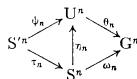
\includegraphics[keepaspectratio]{images/part001_756df219.jpg}}

其中每个箭头表示向量空间同构。若 \(x_{1}, x_{2}, \ldots, x_{n}\) 属于 \(g\)，则 \(\eta_{n}\) 将在 S 中计算的乘积 \(x_{1}x_{2}\ldots x_{n}\) 映到元素

\[
\frac {1}{n !} \sum_ {\sigma \in \mathfrak {S} _ {n}} x _ {\sigma (1)} x _ {\sigma (2)} \dots x _ {\sigma (n)}
\]

该元素在 U 中计算。

推论 5. 设 \(\mathfrak{h}\) 是李代数 \(\mathfrak{g}\) 的子代数，\(\mathrm{U}'\) 是其包络代数。假设 K-模 \(\mathfrak{h}\) 和 \(\mathfrak{g} / \mathfrak{h}\) 是自由的（例如 K 为域时）。令 \(\mathrm{K}\)\((x_{\alpha})_{\alpha \in \mathbb{L}}\) 为 \(\mathfrak{h}\) 的一个基，\((y_{\beta})_{\beta \in \mathbb{M}}\) 为 \(\mathfrak{g}\) 中的一族元素，使它们在 \(\mathfrak{g} / \mathfrak{h}\) 中的典范像构成 \(\mathfrak{g} / \mathfrak{h}\) 的一个基。

\begin{enumerate}
\def\labelenumi{(\alph{enumi})}
\item
  从 \(\mathbf{U}'\) 到 \(\mathbf{U}\) 的典范同态是单射。
\item
  若 \(\mathbf{M}\) 全序，则元素 \(y_{\beta_1} \ldots y_{\beta_q}\)（其中 \(\beta_1 \leqslant \cdots \leqslant \beta_q\)）构成把 \(\mathbf{U}\) 视为 \(\mathbf{U}'\) 的左模或右模时的一个基。
\end{enumerate}

给 \(L \cup M\) 赋予全序，使 L 中每个元素都小于 M 中每个元素。在  中计算的元素 \(x_{\alpha_{1}}x_{\alpha_{2}}\ldots x_{\alpha_{p}}\)（其中 \(U'\)\(\alpha_{1} \leqslant \cdots \leqslant \alpha_{p}\)）构成 \(U'\) 的一个基（推论 3）。元素

\[
x _ {\alpha_ {1}} \dots x _ {\alpha_ {p}} y _ {\beta_ {1}} \dots y _ {\beta_ {q}}
\]

在 U 中计算的这些元素（其中 \(\alpha_{1} \leqslant \cdots \leqslant \alpha_{p} \leqslant \beta_{1} \leqslant \cdots \leqslant \beta_{q}\)）同样构成 U 的一个基。因此，U' 到 U 的典范同态将 U' 的一个基中的元素映到 U 中线性无关的元素，因而是单射。此外可见，\(y_{\beta_1} \ldots y_{\beta_q}\)（其中 \(\beta_{1} \leqslant \cdots \leqslant \beta_{q}\)）构成把 U 视为左 U'-模时的一个基。给  排序，使 M 中每个元素都小于 L 中每个元素，同样可见，\(y_{\beta_1} \ldots y_{\beta_q}\)（其中 \(\beta_{1} \leqslant \cdots \leqslant \beta_{q}\)）构成把 U 视为右 U'-模时的一个基。

在推论 5 的条件下，通过 U' 到 U 的典范同态，将 U' 与 U 中由 h 生成的子代数相同。

推论 6. 假设 K-模 g 是子代数 \(g_{1}, g_{2}, \ldots, g_{n}\) 的直和，且每个 \(g_{i}\) 都是自由 K-模。令 \(U_{i}\) 为 \(g_{i}\) 的包络代数（\(1 \leqslant i \leqslant n\)）。令 \(\phi\) 为从 K-模 \(U_{1} \otimes_{K} \cdots \otimes_{K} U_{n}\) 到 U 的 K-线性映射，它由从  到 U 的多线性映射（\(u_{1}, \ldots, u_{n}\)）\(\mapsto u_{1} \ldots u_{n}\) 定义。则 \(U_{1} \times \cdots \times U_{n}\)\(\phi\) 是 K-模同构。

令 \((x_{\lambda}^{i})_{\lambda \in L_{i}}\) 为 \(g_{i}\) 的一个基。给 \(L_{1} \cup \cdots \cup L_{n}\) 赋予全序，使当  时 \(L_{i}\) 中每个元素都大于 \(L_{j}\)\(i \geqslant j\) 中每个元素。则元素：

\[
\left(x _ {\lambda_ {1}} ^ {1} x _ {\lambda_ {2}} ^ {1} \dots x _ {\lambda_ {p}} ^ {1}\right) \otimes \dots \otimes \left(x _ {\nu _ {1}} ^ {n} x _ {\nu _ {2}} ^ {n} \dots x _ {\nu _ {q}} ^ {n}\right),
\]

其中 \(\lambda_{1}\leqslant\lambda_{2}\leqslant\cdots\leqslant\lambda_{p}\leqslant\cdots\leqslant\nu_{1}\leqslant\nu_{2}\leqslant\cdots\leqslant\nu_{q}\)，构成 \(U_{1}\otimes_{K}\cdots\otimes_{K}U_{n}\) 的一个基。它们经 \(\phi\) 映到元素：

\[
x _ {\lambda_ {1}} ^ {1} x _ {\lambda_ {2}} ^ {1} \dots x _ {\lambda_ {p}} ^ {1} \dots x _ {\nu_ {1}} ^ {n} x _ {\nu_ {2}} ^ {n} \dots x _ {\nu_ {q}} ^ {n}
\]

这些元素构成 U 的一个基。故推论得证。

推论 7. 若 K 是整环且 g 是自由 K-模，则代数 U 没有零因子。

G 与 K 上的多项式代数同构（定理 1），因而是整环（Algebra, Chapter IV, § 1, no. 4, Theorem 1）。故推论成立（Commutative Algebra, Chapter III, § 2, no. 3, Proposition 1）。

\subsection{导子的延拓}

引理 4. 设 V 是 K-模，T 是 V 的张量代数。设 u 是 V 的自同态。存在唯一的延拓 u 的 T 的导子。此导子与 T 上的对称算子交换。

令 \(F = V \times V \times \cdots \times V\)（n 个因子）。映射

\[
\begin{array}{r l} (x _ {1}, \ldots , x _ {n}) & \mapsto u x _ {1} \otimes x _ {2} \otimes \dots \otimes x _ {n} \\ & \qquad + x _ {1} \otimes u x _ {2} \otimes \dots \otimes x _ {n} + \dots + x _ {1} \otimes x _ {2} \otimes \dots \otimes u x _ {n} \end{array}
\]

从 F 到  V 是多线性的。因此存在 \(\bigotimes^{n}\) V 的自同态 \(u_{n}\)\(\bigotimes^{n}\)，使得：

\[
u _ {n} \left(x _ {1} \otimes \dots \otimes x _ {n}\right) = u x _ {1} \otimes \dots \otimes x _ {n} + \dots + x _ {1} \otimes \dots \otimes u x _ {n}
\]

对 V 中所有 \(x_1, \ldots, x_n\) 成立。于是 \(u_1 = u\)。令 v 为 K-模 T 的自同态，它在每个 \(v\) 上与 \(u_n\) 一致，并在 \(\mathrm{T}^n = \bigotimes^n \mathrm{V}\)\(\mathrm{T}^0 = \mathrm{K}. 1\) 上为零。我们证明 v 是 T 的导子。若 \(v\)\(x_1, \ldots, x_n, y_1, \ldots, y_p\) 是 V 的元素，则

\[
\begin{array}{l} v ((x _ {1} \otimes \dots \otimes x _ {n}) \otimes (y _ {1} \otimes \dots \otimes y _ {p})) \\ = \sum_ {i = 1} ^ {n} x _ {1} \otimes \dots \otimes x _ {i - 1} \otimes u x _ {i} \otimes x _ {i + 1} \otimes \dots \otimes x _ {n} \otimes y _ {1} \otimes \dots \otimes y _ {p} \\ \qquad + \sum_ {j = 1} ^ {p} x _ {1} \otimes \dots \otimes x _ {n} \otimes y _ {1} \otimes \dots \otimes y _ {j - 1} \otimes u y _ {j} \otimes y _ {j + 1} \otimes \dots \otimes y _ {p} \\ = v (x _ {1} \otimes \dots \otimes x _ {n}) \otimes (y _ {1} \otimes \dots \otimes y _ {p}) + (x _ {1} \otimes \dots \otimes x _ {n}) \otimes v (y _ {1} \otimes \dots \otimes y _ {p}). \end{array}
\]

\(v\)\(v\)由线性性可知 v 是导子。v 的唯一性是显然的。

最后，显然 \(u_{n}\) 与 \(\otimes V\) 上的所有对称算子交换，因而得到最后一个断言。

命题 7. 设 \(\mathfrak{g}\) 是李代数，U 是其包络代数，\(\sigma\) 是从 \(\mathfrak{g}\) 到 U 的典范映射，D 是 \(\mathfrak{g}\) 的导子。

\begin{enumerate}
\def\labelenumi{(\alph{enumi})}
\item
  存在唯一的 U 的导子 \(\mathrm{D_U}\)，使 \(\sigma \circ \mathrm{D} = \mathrm{D_U} \circ \sigma\)（即当 \(\mathrm{D_U}\)\(\mathfrak{g}\) 在 \(\sigma\) 下可与 U 的一个子模相同时， 延拓 D）。
\item
  \(D_{U}\) 保持 \(U_{n}\) 以及 g 上 n 阶齐次对称张量在 U 中的像的集合 \(U^{n}\) 稳定。
\item
  \(\mathbf{D}_{\mathbf{U}}\) 与 \(\mathbf{U}\) 的主反自同构交换。
\item
  若 \(\mathbf{D}\) 是由 \(\mathfrak{g}\) 的元素 \(x\) 定义的 \(\mathfrak{g}\) 的内导子，则 \(\mathrm{D}_{\mathbf{U}}\) 是由  定义的 \(\mathbf{U}\)\(\sigma(x)\) 的内导子。
\end{enumerate}

令 \(D_T\)\(T\)\(g\)\(D\)\(J\)\(T\) 为延拓 D 的 g 的张量代数 T 的导子（引理 4）。由

\[
x \otimes y - y \otimes x - [ x, y ]
\]

生成的 T 的双边理想 J 在 \((x,y \text{ 属于 } \mathfrak{g})\)\(\mathrm{D}_{\mathrm{T}}\) 下稳定。其中：

\[
\begin{array}{r} \mathrm{D} _ {\mathrm{T}} (x \otimes y - y \otimes x - [ x, y ]) = \mathrm{D} x \otimes y - y \otimes \mathrm{D} x - [ \mathrm{D} x, y ] \\ + x \otimes \mathrm{D} y - \mathrm{D} y \otimes x - [ x, \mathrm{D} y ]. \end{array}
\]

取商后，\(D_{T}\) 定义了 U 的导子 \(D_{U}\)，满足 \(\sigma \circ D = D_{U} \circ \sigma\)。由于 1 和  生成代数 U，\(D_{U}\) 的唯一性是直接的。断言 (b) 是显然的。令 A 为 U 的主反自同构。现在证明 (c)。若 \(\sigma(\mathfrak{g})\)\(x_{1}, \ldots, x_{n}\) 属于 g，则

\[
\begin{array}{r l} \mathrm{D} _ {\mathrm{U}} \mathrm{A} (\sigma (x _ {1}) \dots \sigma (x _ {n})) & = \mathrm{D} _ {\mathrm{U}} ((- 1) ^ {n} \sigma (x _ {n}) \dots \sigma (x _ {1})) \\ & = (- 1) ^ {n} \sum_ {i = 1} ^ {n} \sigma (x _ {n}) \dots \mathrm{D} _ {\mathrm{U}} (\sigma (x _ {i})) \dots \sigma (x _ {1}) \\ & = (- 1) ^ {n} \sum_ {i = 1} ^ {n} \sigma (x _ {n}) \dots \sigma (\mathrm{D} x _ {i}) \dots \sigma (x _ {1}) \\ & = \mathrm{A} \bigg (\sum_ {i = 1} ^ {n} \sigma (x _ {1}) \dots \sigma (\mathrm{D} x _ {i}) \dots \sigma (x _ {n}) \bigg) \\ & = \mathrm{AD} _ {\mathrm{U}} (\sigma (x _ {1}) \dots \sigma (x _ {n})). \end{array}
\]

最后，设 \(x \in \mathfrak{g}\)。令 \(\Delta\) 为 U 的内导子 \(y \mapsto \sigma(x)y - y\sigma(x)\)（Algebra, Chapter IV, § 4, no. 3, Example 2）。则对 \(x' \in \mathfrak{g}\)，

\[
(\Delta \circ \sigma) (x ^ {\prime}) = \sigma (x) \sigma (x ^ {\prime}) - \sigma (x ^ {\prime}) \sigma (x) = \sigma ([ x, x ^ {\prime} ]) = (\sigma \circ \operatorname{ad} x) (x ^ {\prime}),
\]

所以 \(\Delta \circ \sigma = \sigma \circ \operatorname{ad} x\)。证明完毕。

将命题 7 应用于交换李代数的情形可见，K-模的每个自同态 u 都能唯一延拓为该模的对称代数的导子；取商后，此导子由延拓 u 的张量代数导子导出。

再次设 g 是 K 上的李代数，D 是 g 的导子。沿用前面的记号 T、S、U、G。令 \(D_{T}\)、\(D_{S}\) 为分别延拓 D 的 T、S 的导子，令 \(D_{U}\) 为满足 \(\sigma \circ D = D_{U} \circ \sigma\) 的 U 的唯一导子。由于 \(D_{U}\) 保持 \(U_{n}\) 稳定，取商后 \(D_{U}\) 定义了 G 的导子 \(D_{G}\)。由于取商时 \(D_{U}\) 和 \(D_{S}\) 都由 \(D_{T}\) 导出，图 (3) 的交换性表明，\(D_{G}\) 也可由第 6 号定义的同态  从 \(D_{S}\) 导出。若进一步 K 是特征为 0 的域，则图 (4) 的同构将 \(\omega\)\(D_{T}\)、\(D_{S}\)、\(D_{U}\)、\(D_{G}\) 在 \(S^{n}\)、\(S^{n}\)、\(U^{n}\)、\(G^{n}\) 上的限制彼此对应。因此，S 到 U 的典范同构将 \(D_{S}\) 映到 \(D_{U}\)。

\subsection{基环的扩张}

设 g 是 K 上的李代数，T 是其张量代数，J 是由 \(x \otimes y - y \otimes x - [x, y]\)（x, y 属于 g）生成的 T 的双边理想，U = T/J。设 \(K_{1}\) 是含单位元的交换环，\(\sigma\) 是将 1 映到 1 的从 K 到 \(K_{1}\) 的同态。则 \(\mathfrak{g}_{(\mathbf{K}_{1})}\) 的张量代数自然地与 \(\mathrm{T}_{(\mathbf{K}_{1})}\) 相同。令 J' 为由下式生成的 \(J'\)\(\mathrm{T}_{(\mathbf{K}_{1})}\) 的双边理想：

\[
x ^ {\prime} \otimes y ^ {\prime} - y ^ {\prime} \otimes x ^ {\prime} - [ x ^ {\prime}, y ^ {\prime} ]
\]

\((x', y' \text{ 属于 } g_{(K_1)})\)。显然，\(J_{(K_1)}\) 在 \(T_{(K_1)}\) 中的典范像包含于 J'。要看出两者相等，只需证明：若 \(J'\)\(J'\)\(x'\) 和 \(y'\) 表示 \(g_{(K_1)}\) 中的两个元素，则 \(x' \otimes y' - y' \otimes x' - [x', y']\) 属于此像。现在

\[
x ^ {\prime} = \sum_ {i} x _ {i} \otimes \lambda_ {i}, y ^ {\prime} = \sum_ {j} y _ {j} \otimes \mu_ {j} (x _ {i}, y _ {j} \text {   in   } \mathfrak {g}, \lambda_ {i}, \mu_ {j} \text {   in   } \mathrm{K} _ {1});
\]

因此

\[
x ^ {\prime} \otimes y ^ {\prime} - y ^ {\prime} \otimes x ^ {\prime} - [ x ^ {\prime}, y ^ {\prime} ] = \sum_ {i, j} (x _ {i} \otimes y _ {j} - y _ {j} \otimes x _ {i} - [ x _ {i}, y _ {j} ]) \otimes \lambda_ {i} \mu_ {j}
\]

这就证明了断言。于是可见，\(\mathrm{U}_{(\mathbf{K}_{1})} = (\mathrm{T}/\mathrm{J})_{(\mathbf{K}_{1})}\) 自然地与 \(\mathrm{T}_{(\mathbf{K}_{1})}/\mathrm{J}'\) 相同：\(\mathfrak{g}_{(\mathbf{K}_{1})}\) 的包络代数自然地与 \(\mathrm{U}_{(\mathbf{K}_{1})}\) 相同，而 \(\mathfrak{g}_{(\mathbf{K}_{1})}\) 到其包络代数的典范映射与 \(\sigma \otimes 1\) 相同（其中 \(\sigma\) 表示 g 到 U 的典范映射）。

\section{表示}

